%mscS --> seminar
%msc --> Thesis

% برای گزارش سمینار mscS  و برای پایان‌نامه ,msc را انتخاب کنید
\documentclass[oneside,openany,mscS]{SBU-Thesis}

% برای وارد کردن بسته‌هایی که نیاز است قبل از bidi وارد شوند، آنها را در فایل confix.tex قرار دهید. سایر بسته‌های مورد نیاز را در اینجا می‌توانید وارد کنید:

\begin{document}
	%عنوان پایان‌نامه
	\title{بهبود مصرف انرژی در سیستم‌های مبتنی بر اینترنت اشیا}
	
	%رشته
	\subject{مهندسی کامپیوتر}
	
	%گرایش
	\field{نرم‌افزار}
	
	%نام
	\name{پویا}
	
	%نام خانوادگی
	\surname{یارندی}

	%استاد مشاور (در صورت وجود، در غیر این صورت این خط را حذف کنید)
	\firstsupervisor{دکتر محمود نشاطی}

%تاریخ انجام پایان‌نامه
	\thesisdate{تابستان ۱۳۹۹}
	
	%نام دانشکده
	\faculty{دانشکده مهندسی و علوم کامپیوتر}
	
	%نام دانشگاه
	\university{دانشگاه شهید بهشتی}

	% چکیده به فارسی
	\fa-abstract{
امروزه با افزایش قابلیت‌های مبتنی بر اینترنت، نیازمندی بیشتری برای اتصال اشیای پیرامون ما به شبکه اینترنت احساس می‌شود. از این رو، می‌توان گفت مفهوم اینترنت اشیا (\lr{Internet of Things}) روز به روز در حال گسترش است و علاوه بر این، همواره به نیازمندی‌های مبتنی بر اینترنت اشیا افزوده می‌شود. بدیهی است که این افزایش نیازمندی‌ها به پیچیدگی بیشتر سیستم‌های مبتنی بر این فناوری می‌انجامد. بدین سبب می‌توان گفت در آینده با سیستم‌هایی مواجه می‌شویم که پیچیدگی بیشتری دارند. از مصادیق این پیچیدگی می‌توان به گستردگی و دسترس‌پذیری سیستم اشاره کرد. برای مثال؛ زمانی که ما به دنبال ایجاد یک سیستم مبتنی بر اینترنت اشیا برای یک شهر هوشمند هستیم، هزاران حسگر در این سیستم مشغول به مشاهده و پایش محیط خواهند بود و همچنین برای اینکه سیستم ارائه شده، سیستمی مورد اعتماد باشد، لازم است تا دسترس‌پذیری قابل قبولی داشته باشد. یکی از مهم‌ترین عوامل در دست یافتن به دو مورد بالا، بهبود مصرف انرژی در سیستم‌های مبتنی بر اینترنت اشیاست که می‌تواند عمر طولانی‌تر و همچنین هزینه نگهداری کمتری را برای سیستم به ارمغان آورد. در این تحقیق سعی داریم تا با بررسی کارهای صورت گرفته در این زمینه، تکنیک‌های به‌کاررفته در سیستم‌های مبتنی بر اینترنت اشیا را شناسایی کنیم که از این موارد می‌توان به زمان‌بندی فعالیت حسگرها، ارائه توپولوژی بهینه برای شبکه، بهبود ارتباط حسگرها و سایر موارد اشاره کرد. در نهایت نیز، با مقایسه‌ای بین موارد بررسی شده عملکرد تکنیک‌های گوناگون را مورد ارزیابی قرار می‌دهیم. 
	}
	%کلمات کلیدی:
	\keywords{اینترنت اشیا، بهینه‌سازی، مصرف انرژی}
	%%%%%%%%%%%%%%%%%%%%%%%%%%%%%%%%%

%%%%%%%%%%%%%%%%%%%%%
\firstPage
\abstractPage % ساخت صفحه چکیده


\tableofcontents % فهرست مطالب
\listoffigures \newpage % فهرست تصاویر
%\listoftables \newpage % فهرست جداول

%%%%%%%%%%%%%%%%%%%%%%%%%%%

\cchapter{مقدمه}
اینترنت اشیا\LTRfootnote{Internet of Things} یکی از فناوری‌های مورد توجه این روزها در دنیای کامپیوتر است. یکی از عواملی که سبب احساس نیازمندی به این فناوری نوپا گشته، اهمیت یافتن استفاده از اینترنت در دهه اخیر می‌باشد. امروزه نیازمندی انسان به اتصال و بهره‌مندی از شبکه جهانی اینترنت بر کسی پوشیده نیست و حتی بسیاری از نیازهای ابتدایی انسان از طریق اینترنت مرتفع می‌گردد. در چنین شرایطی، برای استفاده از انواع ماشین‌هایی که پیش از این نقش به‌سزایی در بهبود سطح زندگی انسان ایفا می‌کرده‌اند؛ نیازمندی جدیدی حس می‌شد که آن، فعالیت این ماشین‌ها بر بستر اینترنت بود. این امر باعث فعالیت یکپارچه‌تر دستگاه‌هایی می‌شد که پیش از این به طور مستقل از یکدیگر نیازمندی‌های بشر را تامین می‌کردند و بدین سبب، مفهوم اینترنت اشیا معرفی گردید.\\
با گسترش روزافزون نیازمندی‌های مبتنی بر اینترنت اشیا، نیازمندی‌ها و همچنین کاربردهای جدیدی برای این فناوری کشف می‌گردد. برای مثال امروزه شاهد استفاده از سیستم‌های مبتنی بر اینترنت اشیا در کاربرد‌هایی گوناگون همچون ساختمان‌های هوشمند، شهرهای هوشمند و مواردی از این قبیل هستیم. به عنوان مثال، در یک سیستم مبتنی بر اینترنت اشیا که قرار است مدیریت یک شهر هوشمند را برعهده داشته باشد، هزاران حسگر\LTRfootnote{Sensor} در محیطی گسترده (در مقیاس کیلومتر مربع) مشغول به فعالیتند. در چنین شرایطی دو عامل اصلی به عنوان عوامل مورد بررسی جهت سنجش قابل اعتماد بودن\LTRfootnote{Reliability} سیستم مطرح است. این دو عامل دقت مشاهده\LTRfootnote{Observation} محیط و همچنین میزان انرژی مصرفی محیط می‌باشند. در ادامه به بررسی این دو عامل و رابطه‌شان نسبت به یکدیگر می‌پردازیم.\\
یکی از عوامل ذکر شده در بالای برای بررسی میزان قابل اعتماد بودن سیستم‌های مبتنی بر اینترنت اشیا، دقت مشاهده محیط است. فرض کنید در یک خانه هوشمند، قرار است سیستم مراقبت از سالمندان در آن پیاده‌سازی شود. این سیستم باید به طور مداوم به مشاهده محیط پرداخته و در صورت بروز هرگونه رفتار غیرطبیعی در سالمند (از جمله افتادن بر روی زمین و...) اورژانس را از وضعیت به وقوع پیوسته مطلع سازد. علاوه بر این اطلاعاتی از قبیل فشار خون، تعداد ضربان و... نیز از شخص سالمند که در طول چند ساعت اخیر ضبط شده است به سیستم درمانی ارائه دهد. مشخص است که در چنین شرایطی و در چنین سیستمی اهمیت عامل اول، یعنی دقت سیستم بسیار زیاد است.\\
برای دستیابی به چنین هدفی لازم است تا حسگرها به طور مداوم و با فواصل زمانی کم به مشاهده محیط پرداخته و اطلاعات موردنیاز را از محیط جمع‌آوری نمایند. بدین ترتیب، اطلاعات به‌دست‌آمده از محیط، اطلاعات به‌روزتری خواهد بود و به همین دلیل دقت سیستم افزایش می‌یابد. البته به غیر از تناوب مشاهده محیط توسط حسگر‌ها، عوامل دیگری همچون کیفیت خود حسگرها، نحوه نصب آن‌ها در محیط و سایر موارد نیز می‌تواند تاثیر به‌سزایی در دقت اندازه‌گیری مقادیر در محیط و در نتیجه مشاهده بهتر آن داشته باشد که البته این موارد در حیطه بحث این پژوهش نخواهد بود.\\
اما عامل دیگر در بررسی سیستم‌های مبتنی بر اینترنت اشیا که اتفاقا مبحث اصلی این پژوهش نیز بوده، مصرف انرژی\LTRfootnote{Energy consumption} است. یک سیستم مبتنی بر اینترنت اشیا، شامل چندین حسگر است که در محیط مستقر بوده و به تناوب در حال دریافت اطلاعات محیط می‌باشند. بدیهی‌ست که دو موضوع در بحث تامین انرژی حسگرهای چنین سیستمی مطرح است. اول اینکه اگر حسگرهای این سیستم به‌طور بی‌رویه به مشاهده محیط و دریافت اطلاعات از آن بپردازند، انرژی بسیار زیادی مصرف می‌شود که خود این امر تا حدود بسیاری نامطلوب است. به‌هرحال در دنیای امروز یکی از مباحث بسیار مهم و حائز اهمیت، بحث مصرف بی‌رویه منابع انرژی است و واضح است که در صورت بهینه نبودن سیستم‌های مبتنی بر اینترنت اشیا به لحاظ مصرف منابع انرژی، این سیستم‌ها نخواهند توانست جای خود را در زندگی روزمره ما بیابند.\\
علاوه بر این، موضوع دیگری که اهمیت مصرف بهینه منابع انرژی را برای سیستم‌های مبتنی بر اینترنت اشیا دو چندان می‌کند، بحث طول عمر این سیستم‌ها است. با توجه به ماهیت سیستم‌های مبتنی بر اینترنت اشیا، معمولا این سیستم‌ها به لحاظ گستره جغرافیایی سیستم‌هایی بسیار بزرگ هستند که گاها مساحت تحت پوشش آن‌ها می‌تواند به بزرگی یک شهر باشد (همانند مثال شهر هوشمند). بنابراین آنچه حائز اهمیت است، این است که امکان تامین انرژی تمام سیستم به صورت متمرکز ممکن است وجود نداشته باشد. از این روی، رویکرد اصلی در این سیستم‌ها این است که حسگرها خود توانایی تامین انرژی خود را به طور مستقل داشته باشند. یکی از راهکارها در این زمینه، استفاده از باتری برای تامین انرژی حسگرهاست که در جهت مستقل بودن حسگرها و همچنین افزایش قابلیت جابه‌جایی\LTRfootnote{Portability} آن‌ها صورت می‌گیرد. بنابراین منابع انرژی که در اختیار هر حسگر قرار می‌گیرد، محدود است و استفاده بهینه از این منابع بسیار اهمیت می‌یابد. هر چند این منابع قابل تمدید هستند (یعنی می‌توان باتری یک حسگر را با باتری جدید معاوضه نمود.) اما آنچه حائز اهمیت است، در واقع فعال نگه داشتن سیستم برای مدت طولانی تری است. به طور کلی می‌توان طول عمر سیستم را یکی از مزایای بهینه‌سازی مصرف منابع انرژی دانست که منجر به قابل اعتماد بودن بیشتر سیستم می‌گردد.\\
بنابراین همان‌گونه که مشخص است یک \lr{Trade-Off} در بین دقت عملکرد سیستم و طول عمر سیستم وجود دارد. به این معنی که اگر بخواهیم دقت سیستم را افزایش دهیم، حسگرها باید با تناوب‌های زمانی کوتاه‌تری به مشاهده و دریافت اطلاعات محیط بپردازند و در نتیجه انرژی بیشتری مصرف کنند که این امر منجر به کاهش طول عمر حسگرها و در نهایت کاهش طول عمر سیستم می‌گردد. و در طرف مقابل اگر در صدد افزایش طول عمر سیستم‌های مبتنی بر اینترنت اشیا باشیم، بدیهی است که باید تناوب زمانی فعالیت حسگرها طولانی‌تر گردد. این امر باعث می‌شود تا دریافت اطلاعات از محیط با فواصل زمانی بیشتری از جانب حسگرها صورت پذیرد و در نتیجه دقت اطلاعات حاصله از محیط کاهش یابد. چرا که ممکن است تغییراتی در محیط، در فواصل زمانی‌ای رخ دهد که حسگرها مشغول به فعالیت نیستند و در نتیجه برخی اطلاعات در ارتباط با رویدادهای رخ داده در محیط از دست بروند.\\
همان‌طور که مشاهده شد، یک تضاد در میان دو عامل اصلی جهت به‌دست‌آوردن اعتماد برای استفاده از سیستم‌های مبتنی بر اینترنت اشیا وجود دارد. آن‌چه در این تحقیق به آن پرداخته شده است در واقع پدید آوردن توازنی نسبی در میان این دو عامل است. به طوری که یک سیستم مبتنی بر اینترنت اشیا هم دارای دقت قابل قبولی در مشاهده و دریافت اطلاعات مربوط به رویدادهای رخ داده در محیط باشد؛ و هم میزان مصرف منابع انرژی آن بهینه باشد و اتلاف منابع انرژی را به حداقل برساند. برای این منظور پژوهش‌هایی پیش از این صورت گرفته است که ما در این تحقیق به آن‌ها می‌پردازیم. اما به طور کلی چند رویکرد کلی در دستیابی به این امر وجود دارد که در ذیل به شرح مختصری از هر کدام اکتفا می‌کنیم و در بخش‌های بعدی به تفصیل آن‌ها را بررسی می‌نماییم.\\
یکی از رویکردهای پرتکرار در میان مقالات، استفاده از زمانبندی برای فعالیت حسگرهاست. به این معنی که زمان‌های مورد نیاز برای فعالیت یک حسگر مشخص می‌شود و سپس حسگر در این زمان‌ها شروع به فعالیت می‌کند. پس از آن که طبق برنامه زمانبندی شده، زمان فعالیت حسگر به پایان رسید حسگر غیرفعال شده و تا بازه‌ی زمانی بعدی که باید فعالیتش را شروع کند مصرف انرژی خود را به حداقل می‌رساند. این امر اغلب با غیرفعال شدن مدار ارتباطی حسگر صورت می‌گیرد؛ چراکه بخش زیادی از منابع انرژی مصرفی توسط یک حسگر، صرف برقراری ارتباط با دیگر اجزای سیستم می‌گردد. بدیهی است که یکی از دلایل این مصرف زیاد برای برقراری ارتباط این است که اغلب ارتباطات در سیستم‌های مبتنی بر اینترنت اشیا به صورت بی‌سیم\LTRfootnote{Wireless} و با استفاده از تجهیزات ارتباطی نظیر \lr{Bluetooth} صورت می‌پذیرد. در مقالات مختلف دستیابی به یک سیستم زمانبندی برای فعالیت حسگرها، به کمک ابزارهای گوناگون از جمله ارائه معماری برای سیستم‌های مبتنی بر اینترنت اشیا و یا استفاده از مکانیزم های از پیش تعریف شده تحقق یافته است.\\
یکی دیگر از رویکردهای ارائه شده در مقالات مورد بررسی، بحث ارائه یک ساختار جهت برقراری ارتباط میان حسگرها و سایر اجزای سیستم است به طوری که ارتباط آن‌ها با هزینه کمتری به لحاظ مصرف انرژی صورت گیرد. این امر به کمک پیدا کردن مسیرهای کوتاه‌تر در میان اجزای سیستم میسر می‌شود و در واقع اساس کار این رویکردها این است که ارتباط میان اجزای نزدیک به یکدیگر با صرف انرژی کمتری صورت می‌پذیرد. همچنین در این رویکرد، راهکاری برای تجمیع اطلاعاتی که قرار است مورد مخابره قرار گیرد در نظر گرفته شده که از مصرف انرژی بی‌رویه در جهت انتقال اطلاعات در بستر شبکه اینترنت اشیا جلوگیری می‌نماید.\\
در مجموع بعد از بررسی راهکارهای ارائه شده در این پژوهش‌ها مشاهده می‌شود که مصرف انرژی در سیستم‌های مبتنی بر اینترنت اشیا تا مقدار قابل توجهی کاهش یافته و به طور مثال میزان انرژی مصرفی یک سیستم مبتنی بر اینترنت اشیا با ۴۵۰۰ حسگر پس از ۱۲۰ ساعت فعالیت به عددی در حدود $10 \times 10^6 nJ$ کاهش یابد که این مقدار حتی در قیاس با برخی روش‌های دیگر بهینه‌سازی چیزی در حدود ۱/۴ انرژی مصرفی را مورد استفاده قرار می‌دهد.\\
در بخش بعدی گزارش به مروری بر ادبیات تحقیق پرداخته و همچنین اصطلاحات مورد نیاز و همچنین پیش‌زمینه‌های لازم جهت درک بهتر راهکارهای ارائه شده را تشریح می‌نماییم. پس از آن در بخش سوم، به تفصیل، راهکارهای ارائه شده در مقالات مورد بررسی را تشریح کرده و با درخت موضوعی مبحث آشنا خواهیم شد تا ذهنیت مورد نیاز برای زمینه تحقیق را درک نماییم. پس از آن در بخش چهارم به نتیجه‌گیری پرداخته و راهکارهای ارائه شده را با هم مقایسه می‌نماییم و به بیان نقاط ضعف و قوت هریک می‌پردازیم.













\cchapter{مروری بر ادبیات}
در این بخش سعی داریم تا با مروری بر اصطلاحات و ابزارهای مورد استفاده در پژوهش‌های بررسی شده، با پیش‌نیازهای مبحث موردنظر آشنا شویم. 

\section{DRX/DTX}

\begin{figure}
	\centering
	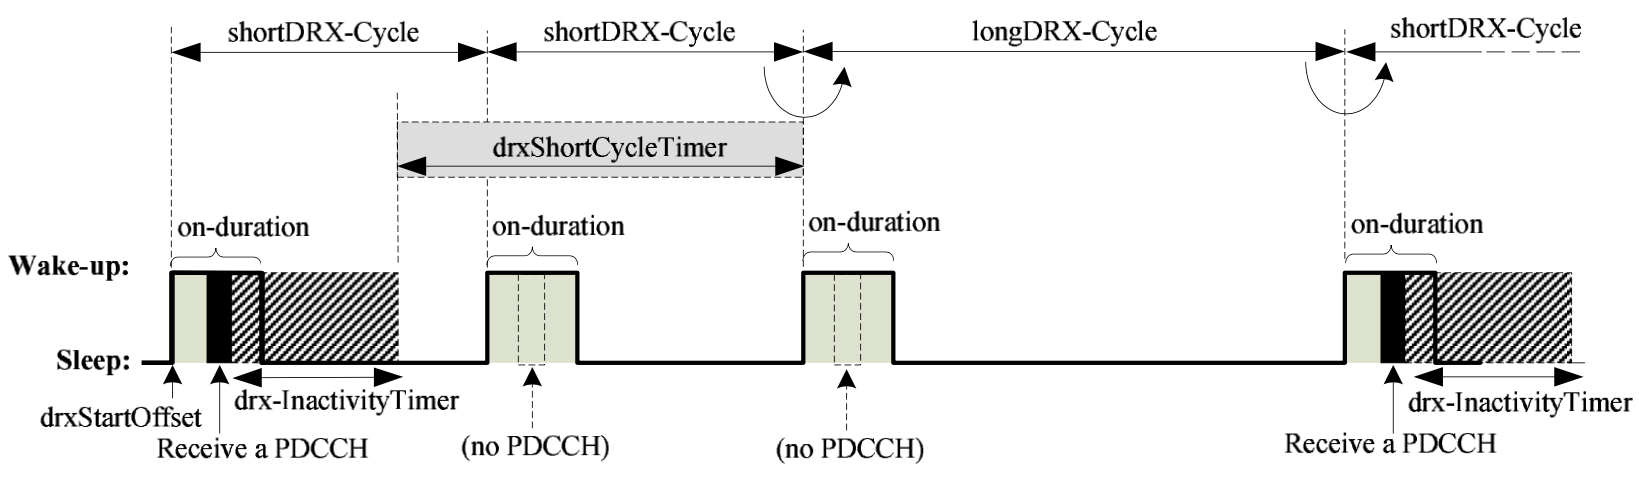
\includegraphics[width=\linewidth]{figs/drx}
	\caption {شمای فعالیت مکانیزم DRX/DTX}
	\label{fig:drx}
\end{figure}

\lr{Discontinuous Reception/Transmission}
یا به اختصار 
\lr{DRX/DTX}
یک مکانیزم از پیش تعریف شده بر بستر شبکه‌های بی‌سیم است که به کمک آن می‌توان زمانبندی فعالیت هر یک از اعضای شبکه (که به اصطلاح، به آن گره\LTRfootnote{Node} نیز گفته می‌شود) ساماندهی نمود. همان‌گونه که در شکل \ref{fig:drx} مشاهده می‌نمایید؛ در شبکه‌هایی که از این مکانیزم استفاده می‌شود در واقع یک چهارچوب خاص برای فعالیت گره‌ها وجود دارد و رفتار ثابت و ازپیش‌تعریف‌شده‌ای را از گره‌ها شاهد هستیم. اما آن‌چه تفاوت در میان گره‌هارا رقم می‌زند مقادیر پارامترهایی است که در این مکانیزم به کار می‌روند. پارامتر‌های \lr{DRX/DTX} هر یک، بیانگر زمان مورد نیاز برای یک رویداد در رفتار گره‌ها هستند. در ادامه به توضیح هر یک از این پارامتر‌ها می‌پردازیم.

\subsection{drxStartOffset}
این پارامتر بیانگر \lr{Offset} زمانی اولیه‌ی پیش از شروع فرآیند توسط گره‌ی شبکه می‌باشد. بدیهی است که تا پیش از این زمان، گره هنوز فعالیت خود را آغاز نکرده است.

\subsection{on-duration}
این پارامتر نمایان‌گر مدت زمانی‌است که پس از هر بار فعال شدن، گره فعال می‌ماند و در انتظار دریافت داده از سایر گره‌ها می‌باشد. گفتنی‌ست که این مدت زمان فعال ماندن یک گره برحسب نیاز می‌تواند افزایش یابد که در ادامه به آن خواهیم پرداخت.

\subsection{drx-InactivityTimer}
پیش‌تر گفتیم که یک گره‌ی شبکه، در زمان خاصی از حالت غیرفعال خارج شده و در انتظار دریافت داده از سایر گره‌های موجود در شبکه می‌ماند. این زمان، در واقع همان زمانی است که در بخش پیش به تعریف آن پرداختیم. اما در آنجا نیز اشاره شد که در صورت دریافت سیگنال از سایر گره‌ها، نیازمند زمان فعالیت بیشتری برای گره هستیم. دلیل آن نیز واضح است. چرا که اگر در اواخر زمان \lr{on-duration}، بسته‌ای (سیگنالی) توسط گره‌ی مذکور دریافت شود، طبیعتا پردازش و در صورت نیاز، پاسخ‌دهی به آن نیازمند زمان است. پس طبق آن‌چه از مرور چنین شرایطی درک می‌نماییم؛ پس از دریافت یک سیگنال، گره نیازمند است تا زمان اضافه‌تری برای فعالیت در اختیار داشته باشد که این زمان اضافه را، \lr{drx-InactivityTimer} می‌نامند. لازم به ذکر است که در این زمان، همان‌طور که از نام این پارامتر نیز مشهود است؛ گره امکان پاسخگویی به درخواست دیگری را ندارد.

\subsection{shortDRX-Cycle}
تمام فرآیندهای ذکر شده در بخش‌های بالا، در یک تناوب مشخصی تکرار می‌شوند که پارامتر \lr{shortDRX-Cycle} بیان‌گر مدت زمان یک دوره می‌باشد. همان‌طور که در شکل \ref{fig:drx} نیز مشاهده می‌شود، طول دوره، به از زمان پارامتر \lr{on-duration} بیشتر خواهد بود. چرا که در هر دوره گره پس از شروع شدن زمان فعالیت، مدتی را منتظر دریافت سیگنال از جانب سایر گره‌ها می‌ماند. پس از این زمان، گره باید قادر باشد تا مدتی را غیرفعال گردد و میزان مصرف انرژی سیستم را کاهش دهد. از این رو، بدیهی است که مدت زمان دوره از زمان فعالیت دستگاه طولانی‌تر باشد.

\subsection{longDRX-Cycle}
پیش از این با مفهوم دوره در شبکه‌های مبتنی بر مکانیزم \lr{DRX/DTX} آشنا شدیم. اما یکی دیگر از جنبه‌های قابل توجه در این مکانیزم، وجود دوره با دو مدت زمان متفاوت است. در این مکانیزم، دو دوره با مدت‌ زمان‌های کوتاه و بلند وجود دارد. فعالیت دستگاه در این سیستم‌ها با دوره کوتاه آغاز می‌شود اما در صورتی که مدتی دستگاه پس از فعال شدن و انتظار دریافت سیگنال، هیچ سیگنالی دریافت نکند؛ در این شرایط وارد دوره‌های بلند مدت می‌شود. از آن‌جا که تمامی پارامتر‌های ذکر شده در بالا برای هر دو طول دوره یکسان است، می‌توان نتیجه گرفت که دوره طولانی‌تر به مدت زمان غیرفعال بودن طولانی‌تری برای دستگاه می‌انجامد و به همین ترتیب میزان مصرف انرژی گره بیش از پیش کاهش می‌یابد.

\subsection{drxShortCycleTimer}
این پارامتر بیانگر مدت زمانی است که پس از آن، دستگاه از دوره‌های کوتاه مدت وارد دوره‌های بلند مدت می‌شود تا انرژی کمتری مصرف نماید.

\begin{figure}
	\centering
	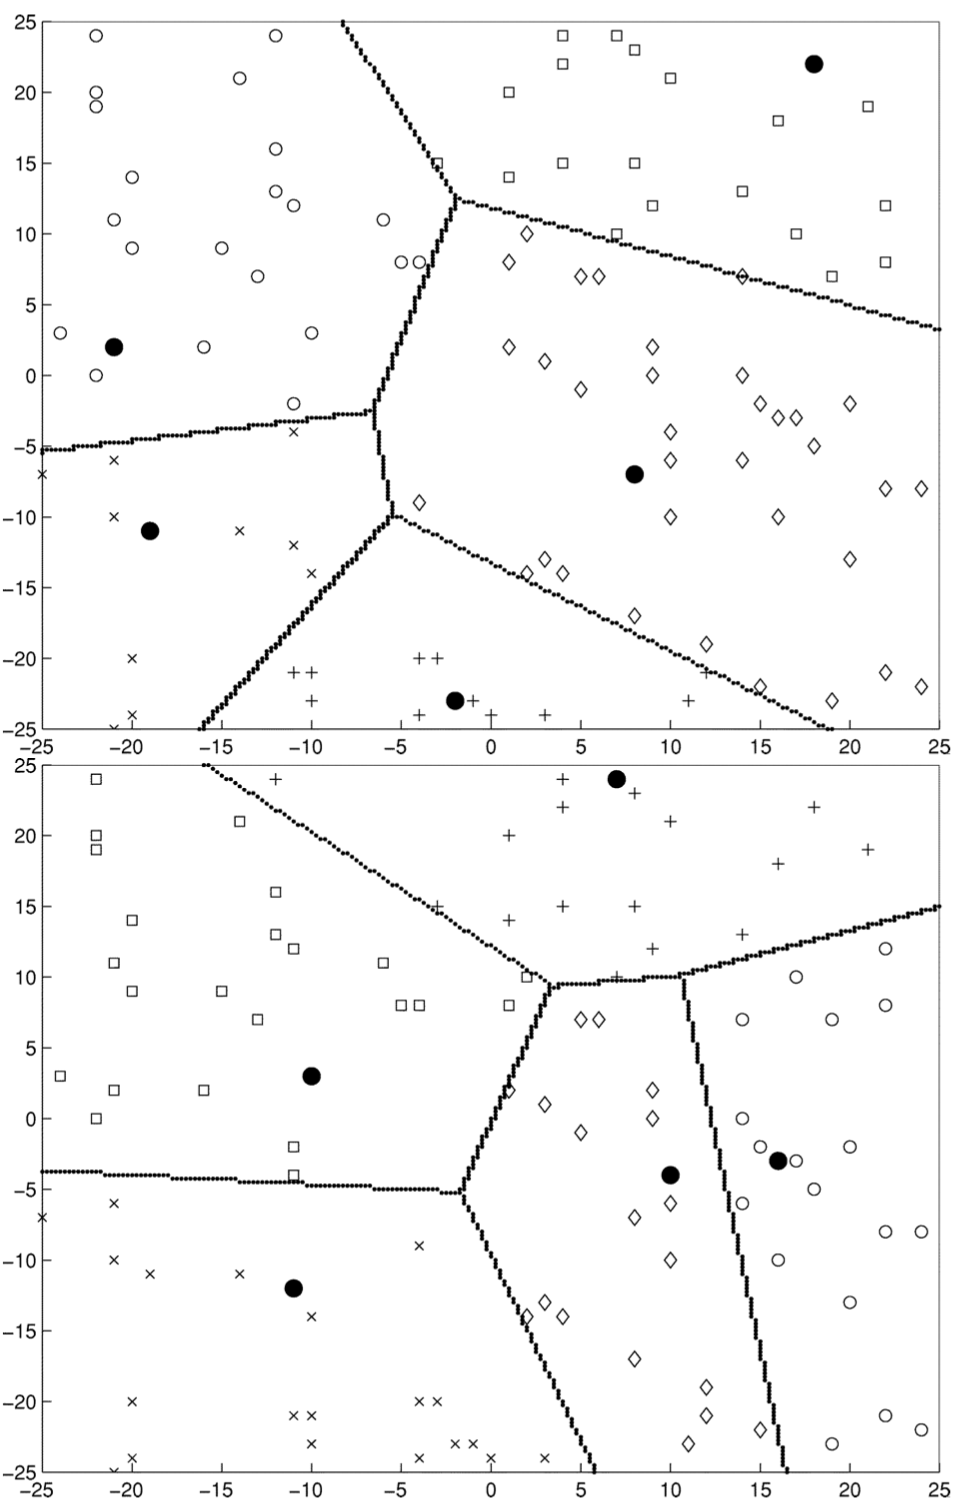
\includegraphics[width=0.7\linewidth]{figs/leach}
	\caption {انتخاب گره‌ی سرگروه و خوشه‌بندی در دو بازه‌ی زمانی متفاوت توسط الگوریتم LEACH}
	\label{fig:leach}
\end{figure}

\section{LEACH}
در مبحث کارهای صورت‌گرفته، در ادامه خواهیم دید که یکی از رویکردها جهت کاهش مصرف منابع انرژی توسط حسگرها در سیستم‌های مبتنی بر رایانش ابری، ارائه گراف یا توپولوژی‌ای برای مشخص نمودن حالت بهینه‌ی ارتباط میان اجزا می‌باشد. در این رویکردها یکی از تکنیک‌های به کار برده شده این است که به دلیل ساختار سلسله‌مراتبی‌شان، در هر حالت، گره‌ای به عنوان گره اصلی خوشه\LTRfootnote{Head node} انتخاب می‌گردد. به طور خلاصه اگر به بیان وظیفه این گره نگاه کنیم؛ در واقع این گره مسئولیت انتقال داده از سطوح بالاتر همچون \lr{Base Station} به حسگرها و همچنین جمع‌آوری داده‌ها از حسگرها و ارسال مجدد آن‌ها برای \lr{Base Station} را بر عهده دارد.
\par
در چنین شرایطی بدیهی است که گره‌ای که به عنوان گره سرگروه خوشه انتخاب می‌گردد؛ دارای فعالیت ارتباطی بیشتری با سایر گره‌ها دارد و در نتیجه منابع انرژی بیشتری را نسبت به سایر گره‌ها مصرف می‌نماید. حال اگر فرض کنیم فرآیند انتخاب گره سرگروه یک فرآیند ثابت باشد - یعنی فقط یک بار گره‌ای را به عنوان سرگروه مشخص کنیم و دیگر آن را تغییر ندهیم - آن‌چه به وقوع می‌پیوندد، این است که در هر خوشه یا منطقه‌ای که مستقلا به عنوان یک گروه در نظر گرفته شده است، یک گره (که همان گره سرگروه است) با مصرف حداکثری انرژی به کار خود ادامه ‌می‌دهد تا زمانی که منابع انرژی خود را به طور کامل مصرف کرده و خاموش گردد. در این رویکرد همان‌طور که قابل مشاهده است، طول عمر سیستم کاهش می‌یابد و این دقیقا در تناقض با یکی از اهداف اصلی ما، یعنی افزایش طول عمر سیستم است.
\par
به همین منظور، الگوریتمی که در مقاله \cite{} معرفی شده است، الگوریتم \lr{LEACH} (مخفف‌شده‌ی عبارت: \lr{Low-Energy Adaptive Clustering Hierarchy}) می‌باشد. رویکرد این الگوریتم به این صورت است که به صورت دوره‌ای، گره سرگروه هر خوشه را تغییر می‌دهد تا سربار انرژی حاصل از برقراری ارتباط میان اجزای سیستم، به طور متوازن میان تمامی گره‌های عضو خوشه تقسیم گردد و در نتیجه، به افزایش طول عمر سیستم منجر شود. در شکل \ref{fig:leach} نمونه ای از رفتار این الگوریتم را در دو دوره‌ی متفاوت زمانی مشاهده می‌کنید.

\section{انواع حسگرها}
همان‌طور که می‌دانیم؛ حسگرهای به کار رفته در یک سیستم مبتنی بر اینترنت اشیا، عمدتا مسئولیت مشاهده و دریافت اطلاعات از محیط را بر عهده دارند و این امر به واسطه‌ی ارتباطشان با \lr{Base Station} و کوئری درخواست شده از جانب آن صورت می‌گیرد. بر این اساس، حسگرهای مبتنی بر اینترنت اشیا، از لحاظ رفتار و نحوه فعالیتشان به دو دسته اساسی تقسیم می‌شوند. این دو دسته عبارتند از:
\begin{itemize}
	\item{حسگرهای Trigger-Based}
	\item{حسگرهای Periodic}
\end{itemize}
\par
در ادامه به تشریح هر یک از انواع مذکور می‌پردازیم.

\subsection{حسگرهای Trigger-Based}
دسته‌ی اول حسگرهای موجود در سیستم‌های مبتنی بر اینترنت اشیا، حسگرهایی هستند که بر اساس یک رویداد خاص در محیط فعال شده و به مشاهده محیط پیرامون می‌پردازند. برای مثال؛ حسگرهای حرکتی از این دست هستند و از کاربردهای مرتبط با آن‌، می‌توان به سیستم‌های روشنایی خودکار محیط اشاره کرد. در این سیستم‌ها با ایجاد حرکت در محیط، حسگر فعال می‌شود و سیگنالی را به \lr{Base Station} تا کنترل‌کننده\LTRfootnote{Controller} سیستم، دستور روشن شدن چراغ‌های موجود در محیط را ارسال کرده و روشنایی محیط تامین شود.

\subsection{حسگر‌های Periodic}
دسته دیگر حسگرهای موجود در سیستم‌های مبتنی بر اینترنت اشیا، حسگر‌های \lr{Periodic} هستند. این حسگرها، فعالیتشان منوط به یک رویداد خاص در محیط نیست و به طور مداوم در حال پایش و مشاهده محیط هستند. برای مثال حسگرهای دمای محیط اغلب به صورت \lr{Periodic} فعالیت می‌کنند. چرا که تغییرات دما در یک محیط عمدتا به صورت پیوسته بوده و همواره در جریان است. اما به این دلیل می‌گوییم اغلب، چرا که حسگر‌های دما نیز می‌توانند به صورت \lr{Trigger-Based} فعالیت کنند و برای مثال؛ صرفا بر اساس تجاوز دما از یک درجه‌ی خاص و یا کاهش دما به میزانی کمتر از حد معین، سیگنال موردنظر را به \lr{Base Station} مخابره نماید تا سیستم، تغییرات خود را بر محیط اعمال کند.

\par
بدیهی است که در یک سیستم مبتنی بر اینترنت اشیا، هر دو نوع حسگرها می‌توانند در کنار یکدیگر به فعالیت بپردازند. یک مثال معروف در این زمینه که در مقاله \cite{} آمده است، مثال مدیری است که برای جلسه فردا برنامه‌ریزی می‌کند. در این مثال بیان می‌شود که یک مدیر، برای جلسه فردای خود که در ساعت هشت صبح است ساعتش را کوک می‌کند تا در ساعت ۷ صبح بیدار شود. در این بین، در ساعت ۶:۳۰ صبح گوشی مدیر با چک کردن داده‌های مربوط به ترافیک متوجه ترافیک سنگین می‌شود و مدیر را زودتر بیدار می‌کند. پنج دقیقه بعد، زمانی که مدیر در حال استحمام است؛ سیستم، دستور فعال شدن را برای دستگاه چای‌ساز صادر می‌کند تا در هنگام آماده شدن مدیر چای، آماده باشد و چای‌ساز در زمانی که چای آماده می‌شود، سیگنالی را به سیستم میفرستد تا سیستم از این رویداد آگاه گردد. در این همین مثال مشاهده می‌شود که هر دو نوع حسگرهای \lr{Trigger-Based} و \lr{Periodic} در حال فعالیت در کنار یکدیگر می‌باشند. برای مثال؛ حسگر موجود در دستگاه چای‌ساز به صورت \lr{Trigger-Based} عمل می‌نماید. حال آن‌که گوشی - که به عنوان حسگر ترافیک در سیستم مشغول به کار است - به صورت \lr{Periodic} فعال است. نکته دیگر در تفاوت میان این دو نوع حسگر این است که به طور معمول، حسگرهای \lr{Periodic} اطلاعات کاملی را از محیط مورد پایش خود به کنترل‌کننده ارائه می‌کنند. در صورتی که در اغلب موارد، حسگرهای \lr{Trigger-Based} صرفا یک سیگنال را که بیانگر وقوع رویداد است مخابره می‌کنند و این سیگنال شامل پارامترهای اضافی نیست.

\section{خودسازماندهی}
یکی از مفاهیم به کار رفته در مقاله \cite{} که در فصل بعدی به تفصیل به آن خواهیم پرداخت، خودسازماندهی\LTRfootnote{Self-Configuration} است. خودسازمندهی به معنی توانایی سیستم به ایجاد تغییر در رفتار خود به منظور بهبود عملکرد سیستم بوده و شامل جنبه‌های گوناگونی است که در ادامه به توضیح مختصری از هر یک می‌پردازیم. لازم به ذکر است؛ تعاریف ارائه شده در مقاله مذکور هیچ یک به تنهایی چرخه \lr{MAPE} را به وجود نمی‌آورند. اما از مجموعه این اعمال چرخه\lr{MAPE} پدید خواهد آمد. چرخه \lr{MAPE} یک چرخه تکاملی است که در سیستم‌های خودسازمانده وجود دارد و حرکت سیستم در راستای این چرخه منجر به خودمختاری سیستم می‌گردد. این چرخه شامل چهار مرحله زیر است. در شکل \ref{fig:mape} می‌توانید این چرخه را مشاهده نمایید. 
\begin{itemize}
	\item{$Monitoring$ به معنی مشاهده و پایش محیط و دریافت اطلاعات از آن.}
	\item{$Analayze$ به معنی دریافت اطلاعات و پردازش آن‌ها که منجر به درک سیستم از محیط می‌گردد.}
	\item{$Planning$ به معنی تصمیم‌گیری برای ایجاد تغییرات بر روی محیط براساس دانش موجود در ارتباط آن.}
	\item{$Execution$ اعمال تغییرات برنامه ریزی شده در مرحله قبلی براساس ارسال دستورات به عمل‌کننده‌های محیطی.}
\end{itemize}
\par
در مقاله مذکور سه اصل جهت ایجاد چنین چرخه‌ای ذکر شده است که این مراحل به شرح زیر ‌می‌باشند.
\begin{itemize}
	\item{خودپیکربندی\LTRfootnote{Self-Configuration}}
	\item{خودبهینگی\LTRfootnote{Self-Optimization}}
	\item{خودالتیامی\LTRfootnote{Self-Healing}}
\end{itemize}

\begin{figure}
	\centering
	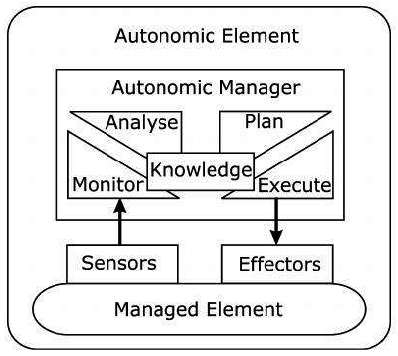
\includegraphics[width=0.5\linewidth]{figs/mape}
	\caption {چرخه MAPE}
	\label{fig:mape}
\end{figure}

\subsection{خودپیکربندی}
خودپیکربندی یک ویژگی در سیستم‌های خودمختار است که به واسطه‌ی آن، یک موجودیت جدید که در این سیستم وارد می‌شود نیازمند تنظیمات اولیه برای قرار گرفتن در جریان کاری سیستم نیست و توسط خود سیستم پیکربندی اولیه برای آن صورت می‌گیرد. این ویژگی به کاهش خطای انسانی به هنگام پیکربندی اولیه اجزا و البته کاهش پیچیدگی در سیستم منجر می‌شود.

\subsection{خودبهینگی}
خودبهینگی، ویژگی دیگری در سیستم‌های خودمختار است که به واسطه‌ی آن، سیستم با اعمال تغییرات در پارامترهای موجود در اجزا، سعی در بهینه‌سازی عملکرد کلیت سیستم خواهد داشت. در مقاله \cite{}، این شاخصه، به کمک یک تابع پیاده‌سازی شده است که وظیفه‌ی آن تعیین وضعیت فعالیت هر حسگر می‌باشد. در فصل بعدی به تفصیل این تابع را مورد تشریح قرار خواهیم داد.

\subsection{خودالتیامی}
دیگر ویژگی سیستم‌های خودمختار، خودالتیامی می‌باشد. خودالتیامی بیان‌گر رفتاری در سیستم است که منجر به یافتن خطاهای سیستم و رفع کردن آن‌ها می‌گردد. در مقاله مورد بحث پس از طی مراحل قبلی که منجر به پیکربندی و سپس تعیین حالت حسگرها می‌شود؛ این ویژگی منجر به اصلاح وضعیت هریک از حسگرها در صورت لزوم خواهد شد. این تابع نیز در فصل بعد به طور کامل مورد بررسی قرار خواهد گرفت و با عملکرد آن آشنا خواهیم شد.

\section{پارامترهای اندازه‌گیری}
در سیستم‌های مبتنی بر اینترنت اشیا، و اصولا به طور کلی، در هر سیستم پیاده‌سازی شد؛ یکی از مهم‌ترین دغدغه‌ها در ارتباط با صحت عملکرد سیستم پیشنهادی است. در این میان، در بین مقالاتی که مورد بررسی قرار گرفت، تعدادی از این پارامترها به عنوان پارامتر‌های اندازه‌گیری در جهت اثبات کارکرد راهکار پیشنهادی مورد استفاده قرار گرفته است. در ادامه این بخش به تشریح برخی از این پارامترها می‌پردازیم.

\subsection{\lr{Packet Loss Rate}}
یکی از پارامتر‌های اندازه‌گیری که در بررسی عملکرد سیستم‌های مبتنی بر اینترنت اشیا به کار می‌رود؛ \lr{Packet Loss Rate} است. همان‌طور که می‌دانیم، اساس کار سیستم‌های مبتنی بر اینترنت اشیا، ارسال و دریافت پیام میان حسگرها و واحد کنترل‌کننده است. این پیام‌های در قالب بسته\LTRfootnote{Packet}هایی از داده بین اجزای سیستم منتقل می‌گردند و بنابر برخی عوامل ممکن است ارسال و یا دریافت آنان از جانب فرستنده و یا گیرنده دچار مشکل شود که در چنین حالتی ارسال پیام ناموفق بوده است. این پارامتر، بیانگر نسبت پیام‌های ارسالی ناموفق به مجموع پیام‌های مخابره شده در سیستم است.

\subsection{Jitter}
یکی دیگر از پارامتر‌های به کار رفته در مقالات مورد بررسی، \lr{Jitter} \cite{} می‌باشد. \lr{Jitter} در واقع، از محاسبه انحراف معیار مدت‌زمان دریافت بسته‌های ارسالی، به دست می‌آید. به عبارتی می‌توان دلیل اهمیت این پارامتر را در این دانست که اگر در بین مدت‌زمان‌های ثبت شده، بنابر هر دلیلی یکی از بسته‌ها با تاخیر قابل‌توجهی در دریافت مواجه شد؛ این امر کل عملکرد سیستم را از لحاظ ارزیابی تحت‌الشعاع قرار ندهد.

\subsection{\lr{Average Sleep Ratio}}
یکی دیگر از پارامترهای مورداستفاده، میانگین نسبت غیرفعال بودن\LTRfootnote{Average Sleep Ratio} سیستم است. همان‌گونه که از نام این پارامتر مشخص است؛ از میانگین نسبت زمان غیرفعال بودن حسگرها به نسبت به کل زمان فعالیت سیستم به‌دست می‌آید.

\par
لازم به ذکر است که پارامتر‌های اندازه‌گیری نام‌برده شده در بالا، تمام پارامترهای مورد استفاده در مقالات مورد بحث نیستند. ما در این‌جا پارامترهایی را مورد بحث قرار داده‌ایم که نیازمند تشریح بیشتر بوده‌اند و در صورت نیاز، بقیه‌ی پارامتر‌ها را در فصل بعد، به طور ضمنی و به‌طور خلاصه تعریف می‌نماییم.

\section{\lr{IEEE 802.15.4}}
\lr{IEEE 802.15.4}
یک استاندارد ارتباطی کوتاه‌برد همانند \lr{Bluetooth} است با این تفاوت که به لحاظ مصرف انرژی بهینه‌تر از این فناوری می‌باشد. این استاندارد که لایه‌ی فیزیکی و \lr{Media Access Control} را در سیستم مشخص می‌نماید؛ به طور ذاتی برای کار با پروتکل آدرس‌دهی \lr{IPv4} طراحی شده است. اما برای این‌که قابلیت استفاده از پروتکل آدرس‌دهی \lr{IPv6} را نیز داشته باشد می‌توان از یک تبدیل‌گر به نام
\lr{6LoWPAN} \RTLfootnote{مخفف \lr{IPv6 over Low Power Wireless Personal Area Networks}}
استفاده نمود که وظیفه‌ی آن فشرده کردن سربار\LTRfootnote{Overhead} بسته‌های ارسالی با استفاده از این پروتکل است تا با سرباری فشرده‌تر امکان انتقال این بسته‌ها بر بستر یک شبکه‌ی مبتنی بر \lr{IEEE 802.15.4} وجود داشته باشد. اما ما به دلیل آن‌که این مبحث در چهارچوب کلی بحثمان نیست از تشریح بیشتر آن صرف‌نظر کرده و به همین تعریف کوتاه اکتفا می‌نماییم.

\section{IPv6}
برای تعریف این مفهوم ابتدا لازم است به طور کلی در ارتباط با پروتکل آدرس‌دهی به بحث بپردازیم. وظیفه‌ی اصلی پروتکل‌های آدرس‌دهی تخصیص یک شناسه‌ی یکتا به دستگاه‌های موجود در یک شبکه است که به کمک این شناسه قابلیت قابلیت شناسایی دستگاه‌ها و همچنین مکان‌یابی آن‌ها وجود داشته باشد. در همین زمینه، ابتدا \lr{IPv4} معرفی شد که پس از مدتی در سال ۱۹۹۰ و با افزایش سرعت فراگیر شدن اینترنت، دانشمندان حوزه‌ی شبکه به این حقیقت پی بردند که میزان شناسه‌های یکتا برای شبکه‌ی اینترنت بسیار بیشتر از آن چیزیست که ‌\lr{IPv4} ارائه می‌دهد. در همین راستا بود که \lr{IPv6} ابداع شد.

\par
\lr{IPv6}
بر خلاف \lr{IPv4} که ساختاری ۳۲ بیتی داشت، ساختاری ۱۲۸ بیتی دارد. به این معنا که در تئوری توانایی تولید $2^{128}$ شناسه یکتا را دارد. این رقم چیزی در حدود $3.4 \times 10^{38}$ شناسه می‌شود که می‌توان گفت حدودا $7.9 \times 10^{28}$ برابر تعداد شناسه‌های قابل تولید توسط \lr{IPv4} می‌باشد.

\par
اما صرف‌نظر از برتری \lr{IPv6} از لحاظ تعداد بیشتر شناسه‌های یکتای تولیدی نسبت به \lr{IPv4}، یک برتری دیگر نیز در این نسخه از پروتکل آدرس‌دهی مذکور وجود دارد و آن هم ویژگی خودپیکربندی است. به واسطه این ویژگی جدید، دستگاه‌هایی که به شبکه افزوده می‌شوند، برای دریافت شناسه‌ی یکتا (یا همان \lr{IP}) نیازی به ارتباط با یک سرور 
\lr{DHCP}\RTLfootnote{مخفف \lr{Dynamic Host Configuration Protocol}}
ندارند. واضح است که این ویژگی تا چه میزان می‌تواند در سیستم‌های مبتنی بر اینترنت اشیا کاربردی باشد؛ چراکه در این سیستم‌ها به طور معمول با حجم عظیمی از تجهیزات و حسگرها مواجه هستیم که نیازمند پیکربندی می‌باشند. همین امر مهم می‌تواند \lr{IPv6} را به یکی از راهکاری اصلی برای پروتکل آدرس‌دهی در سیستم‌های مبتنی بر اینترنت اشیا تبدیل نماید.

\par
حال که به طور اجمالی با عبارات، ابزارها و فناوری‌های مورد استفاده در مقالات تحت بررسی آشنایی یافتیم؛ در فصل بعد به بیان ‌ایده‌های مطرح شده در این مقالات می‌پردازیم. شایان ذکر است که در این بخش، سعی شد تا به حداکثر مباحث پیش‌نیاز پرداخته شود. اما ممکن است برخی اصطلاحات به‌کار رفته در فصول بعدی، در این بخش مورد بحث واقع نشده باشد؛ که در این صورت در همان فصول و به اختصار به شرح و مرور آن‌ها خواهیم پرداخت.











\cchapter{کارهای مرتبط}

\begin{figure}
	\centering
	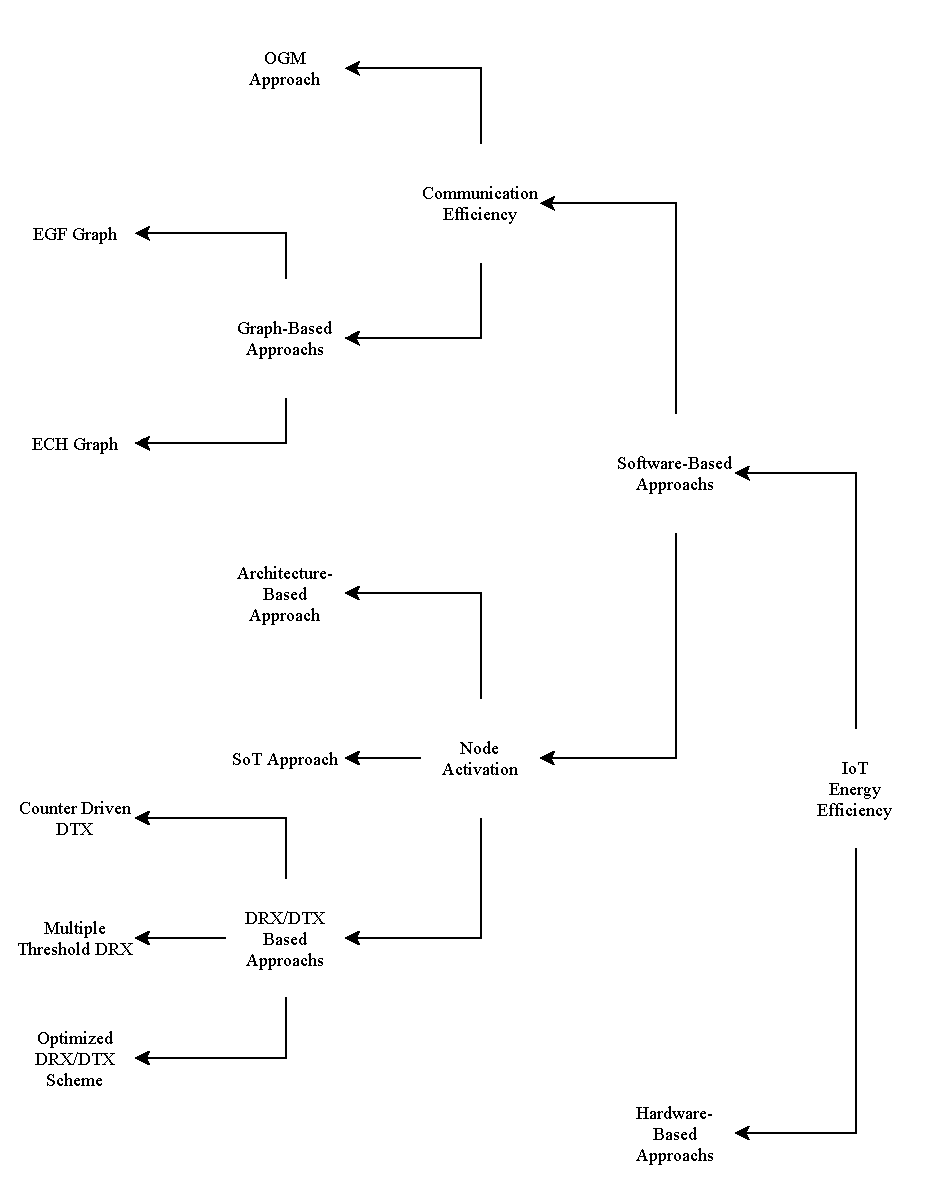
\includegraphics[width=0.9\linewidth]{figs/subject-tree}
	\caption {درخت موضوعی تحقیق}
	\label{fig:subject-tree}
\end{figure}

\par
در این بخش به بیان ایده‌های مطرح شده در مقاله‌های تحت‌بررسی می‌پردازیم. شکل \ref{fig:subject-tree} نمایان‌گر درخت موضوعی تحقیق است و همان‌طور که در تصویر مشاهده می‌نمایید؛ اساسا راهکارهای ارائه شده برای کاهش مصرف انرژی در سیستم‌های مبتنی بر اینترنت اشیا، به دو دسته‌ی کلی راهکارهای نرم‌افزاری و سخت‌افزاری تقسیم می‌گردد. در راهکارهای نرم‌افزاری، دو ایده‌ی اصلی مطرح بوده است که این ایده‌ها به ترتیب هدفشان بهینگی ارتباطات میان اجزای سیستم به منظور کاهش اتلاف انرژی در جریان انتقال داده‌ها و دیگری، غیرفعال نمودن اجزا (در این‌جا بیشتر منظور حسگرها می‌باشند.) در شرایط غیرضروری جهت کاهش مصرف انرژی توسط آن‌ها است.
\par
برای رویکرد، اول در برخی مقالات، روش‌های مبتنی بر گراف معرفی شده است که بهینگی ارتباطات سیستم را مورد هدف قرار داده‌اند. در ارتباط با رویکرد دوم نیز، معماری‌هایی ارائه شده که در آن‌ها فعال و یا غیرفعال بودن حسگرها بنابر ایده‌ی ابتکاری ارائه شده تعیین می‌گردد. علاوه بر معماری‌های ارائه شده، در برخی مقالات از مکانیزم \lr{DRX/DTX} برای فعال و غیرفعال نمودن حسگرها استفاده شده است. در ادامه به بررسی و تشریح هر یک از راهکارهای زیر خواهیم پرداخت.

\section{راهکارهای مبتنی بر مکانیزم \lr{DRX/DTX}}
پیشتر در ارتباط با مکانیزم \lr{DRX/DTX} به تفصیل صحبت کرده‌ایم. حال می‌خواهیم مقالاتی را که از این مکانیزم در بیان راهکارهایشان استفاده کرده‌اند، مورد بررسی قرار دهیم.

\subsection{\lr{Counter Driven DRX (CDD)}}
اولین راهکاری که مورد بررسی قرار می‌دهیم، راهکاری است که در مقاله \cite{} مطرح گردیده. همانطور که پیشتر نیز گفتیم، یک \lr{Trade-Off} مابین مصرف انرژی و دقت سیستم وجود دارد که می‌توان گفت این مقاله سعی در جهت ایجاد توازن در این امر را دارد. در این مقاله، هر یک از گره‌ها برای ارتباط با گره دیگر، دارای دو شمارنده هستند. در ادامه نحوه عملکرد هر یک از آن‌ها را تشریح می‌نماییم.
\par
برای بیان نحوه کارکرد این شمارنده‌ها لازم است ابتدا با نحوه عملکرد اجزای سیستم آشنایی یابیم. در یک سیستم مبتنی بر \lr{DRX/DTX}، یک گره در زمان معینی بیدار می‌شود (فعالیت خود را آغاز می‌کند)، در زمانی که فعال است به درخواست‌های رسیده از جانب دیگر گره‌ها پاسخ می‌دهد و پس از پایان زمان فعالیت مجددا به خواب می‌رود (غیرفعال می‌شود). حال اگر گره، در زمانی از خواب بیدار شود و در تمام طول مدتی که فعال است درخواستی از جانب دیگر گره‌ها دریافت ننماید، شمارنده‌ی اول خود را افزایش می‌دهد. اما اگر در یکی از زمان‌های فعالیت، گره درخواستی از دریافت نماید این شمارنده به مقدار اولیه (یا همان صفر) \lr{Reset} می‌گردد. پس از آن‌که مقدار این شمارنده از یک حدحساب\LTRfootnote{Threshold} عبور کرد؛ زمان دوره \lr{DRX} افزایش می‌یابد. همان‌طور که در فصل قبل نیز به آن اشاره شد، با افزایش زمان دوره در این مکانیزم، در واقع زمان فیرفعال بودن گره افزایش می‌یابد. در نتیجه این سیستم در واکنش به کمبودن در خواست برای یک گره (یا همان حسگر)، فعالیت آن را کاهش داده تا در مصرف انرژی صرفه‌جویی نماید. در شکل \ref{fig:cdd-extend} نمونه فعالیت این راهکار را برای افزایش زمان غیرفعال بودن یک گره مشاهده می‌کنید.

\begin{figure}
	\centering
	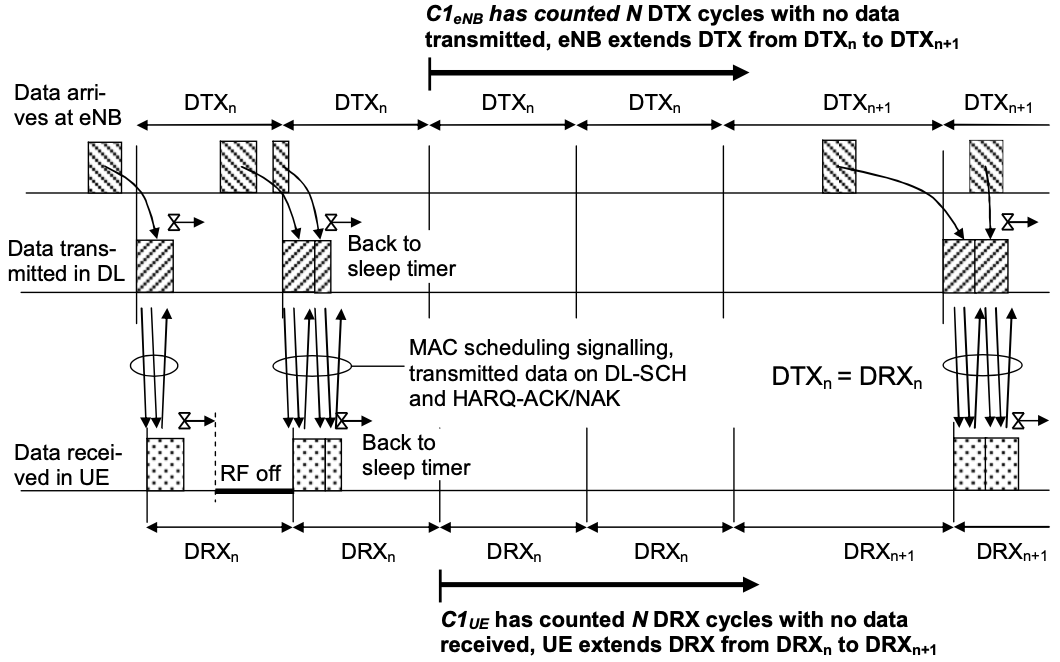
\includegraphics[width=0.7\linewidth]{figs/cdd-extend}
	\caption {افزایش دوره DRX در واکنش به کمبود درخواست برای گره}
	\label{fig:cdd-extend}
\end{figure}

\begin{figure}
	\centering
	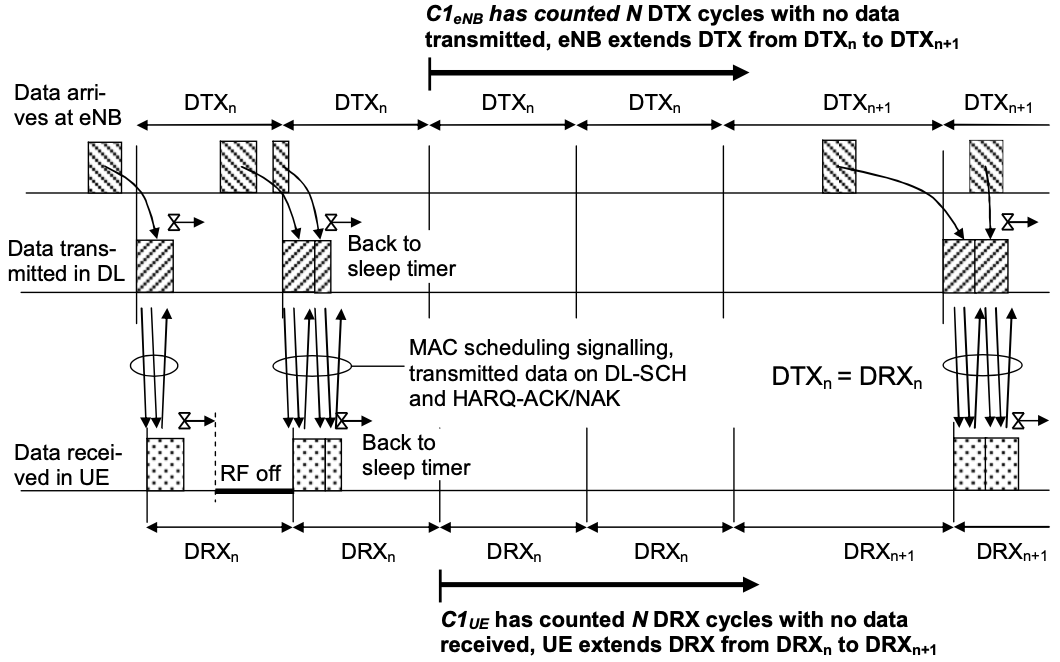
\includegraphics[width=0.7\linewidth]{figs/cdd-extend}
	\caption {کاهش دوره DRX در واکنش به ازدیاد درخواست برای گره}
	\label{fig:cdd-reduce}
\end{figure}

\par
تا این‌جا رویکرد راهکار ارائه شده در واکنش به عدم نیاز به جمع‌آوری داده از یک حسگر را دیدیم. حال به بررسی دومین شمارنده می‌پردازیم. در این شمارنده که به نوعی می‌توان گفت عکس عمل شمارنده‌ی اول را انجام می‌دهد؛ در هر دوره که گره، بیدار می‌شود؛ در صورتی که در زمان بیداری درخواستی جهت پاسخگویی به گره ارسال شده باشد، شمارنده یک واحد افزایش می‌یابد و در صورتی که درخواستی برای گره ارسال نشود، مقدار شمارنده به صفر \lr{Reset} خواهد شد. همانند شمارنده‌ی قبل؛ برای این شمارنده نیز حدحسابی درنظر گرفته شده است که اگه مقدار شمارنده از این حدحساب عبور کند، دوره تناوب گره کاهش می‌یابد. همان‌طور که گفته شد، این عمل برعکس عمل شمارنده‌ی بالاست. یعنی به کمک این شمارنده، سیستم متوجه می‌شود که گره در هر دوره‌ی بیداری درخواستی برای پاسخگویی داشته و در نتیجه، سیستم درمی‌یابد که نیازمندی سیستم به این گره بیش از مقدار فعلی است. پس برای افزایش دقت سیستم لازم است تا گره با تناوب کوتاه‌تری به فعالیت بپردازد  که البته همان‌طور که پیشتر هم اشاره شده این امر موجب افزایش انرژی مصرفی گره و در ازای آن، کاهش طول عمر سیستم می‌شود. در شکل \ref{fig:cdd-reduce} نمونه فرآیند کاهش طول دوره برای یک گره را مشاهده می‌نمایید.

\subsubsection{نیرومندی راهکار ارائه شده}
منظور از نیرومندی\LTRfootnote{Robustness} راهکار ارائه شده، اثبات عملکرد آن در ازای بروز هرگونه خطا می‌باشد. به همین منظور، در مقاله مذکور مجموعا چهار نوع خطا در حین کارکرد سیستم ارزیابی شده است. که به شرح ذیل می‌باشند.
\begin{enumerate}
	\item{
	گره درخواست‌کننده، درخواست را زمانبندی می‌کند. اما در ارسال موفق نمی‌شود. گره پاسخگو، سیگنال منفی (\lr{NAK}) در پاسخ می‌فرستد.
	}
	\item{
	گره درخواست‌کننده، درخواست را زمان‌بندی و ارسال می‌کند. گره پاسخگو، سیگنال را با خطا می‌فرستد.
	}
	\item{
گره درخواست‌کننده، برای ارسال درخواست دچار خطا می‌شود و گره پاسخگو نیز در ارسال سیگنال پاسخ دچار خطا می‌گردد.
	}
	\item{
گره درخواست‌کننده، در زمان‌بندی و ارسال درخواست دچار خطا می‌شود و طبیعتا به دلیل خطای زمان‌بندی، امکان ارسال سیگنال از جانب گره پاسخگو وجود ندارد.
	}
\end{enumerate}

\par
خطاهای ذکر شده در بالا را می‌توانید در شکل \ref{fig:cdd-errors} مشاهده نمایید. همانگونه که در تصویر نیز مشهود است؛ در صورت بروز هر یک از خطا دو سیستم از نقطه $A$ به بعد مجددا با هم همگام شده و عملکرد طبیعی سیستم مشاهده می‌گردد.

\begin{figure}
	\centering
	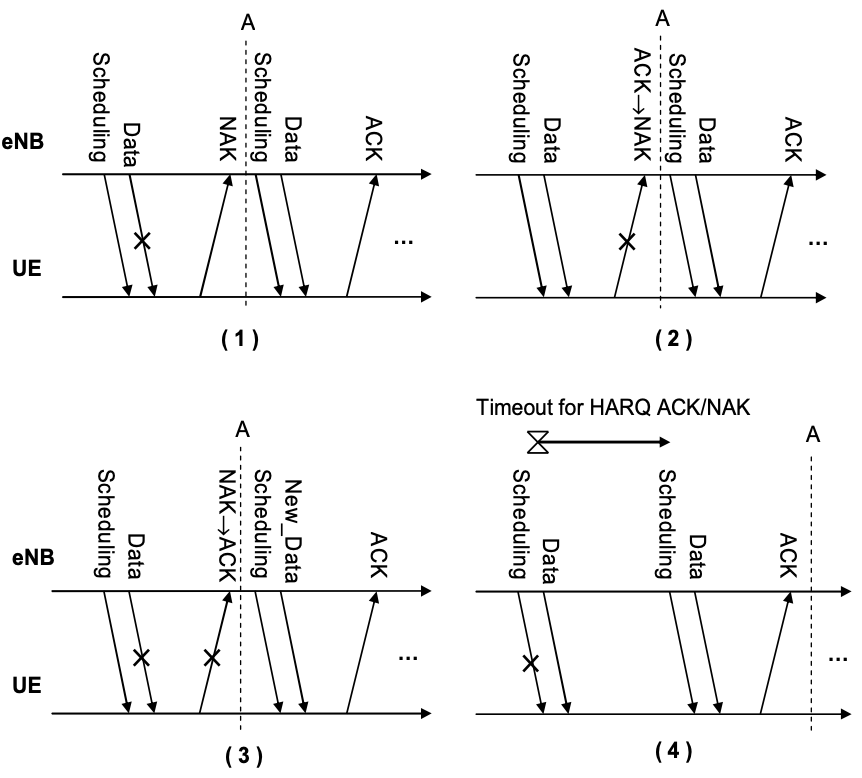
\includegraphics[width=0.8\linewidth]{figs/cdd-errors}
	\caption {خطاهای ممکن در حین برقرار ارتباط میان دو گره}
	\label{fig:cdd-errors}
\end{figure}

\subsection{\lr{Multiple Threshold DRX (MTD)}}
راهکار ارائه شده در این مقاله\cite{}، این است که برخلاف راهکار ارائه شده در مقاله‌ی قبل، تغییری در طول دوره‌ی گره ایجاد نمی‌شود؛ بلکه بر اساس شیوه‌ای به تغییر مقدار زمان \lr{Inactivity Timer} گره می‌پردازد. در مورد این پارامتر نیز در فصل پیش به تفصیل صحبت کردیم اما برای یادآوری، این پارامتر بیانگر مدت زمانی بود که گره، پس از دریافت درخواست از جانب سایر گره‌ها روشن می‌ماند تا درخواست رسیده را پاسخ دهد و در این مدت به سایر درخواست‌های رسیده پاسخگو نبود.
\par
در راهکار ارائه شده در مقاله مورد بررسی، ۱۰ حالت برای کیفیت عملکرد گره‌ها در نظر گرفته شده است که از حالت ۱ الی ۱۰ زمان \lr{Inactivity Timer} آن‌ها افزوده شده و در نتیجه کیفیت عملکرد آن‌ها کاهش می‌یابد. دلیل کاهش کیفیت عملکرد از دیدگاه این مقاله، این است که با افزایش زمان \lr{Inactivity Timer}، امکان دریافت درخواست‌های جدید از گره سلب می‌شود و دقت کاهش می‌یابد. پس در نتیجه، حالت ۱ باکیفیت‌ترین و حالت ۱۰ کم‌کیفیت‌ترین حالت است. این حالات را می‌توانید در جدول \ref{tbl:mtd} مشاهده نمایید. در ابتدا، تمامی گره‌ها در حالت ۱ قرار دارند. پس از آن‌، به طور متاوب، شاخص کیفیت (\lr{CQI}\RTLfootnote{مخفف \lr{Channel Quality Indicator}}) هر یک از گره‌ها محاسبه می‌شود.
پس از محاسبه‌ی \lr{CQI} هریک از حالات مذکور دارای یک حدحساب \lr{CQI} است که این حدحساب‌ها در شکل \ref{fig:mtd} قابل‌مشاهده است. اگر در مدت‌زمان $T\_trig$ که در جدول \ref{tbl:mtd} آمده است، مقدار \lr{CQI} پایین‌تر از حدحساب باشد، گره از حالت فعلی به یک حالت بالاتر می‌رود و در نتیجه تایمر طولانی‌تر شده که منجر به کاهش کیفیت عملکرد و البته، افزایش طول عمر گره می‌گردد.
\par
برعکس همین عمل نیز در سیستم اتفاق می‌افتد. یعنی اگر برای یک گره، در ازای مدت‌زمان بیشتری از $T\_trig$ میزان \lr{CQI} بالاتر از حدحساب حالت کمتر (باکیفیت‌تر) باشد، حالت کیفیت گره به حالت باکیفیت‌تر تقلیل می‌یابد که موجب افزایش دقت عملکرد حسگر می‌گردد.

\begin{figure}
	\centering
	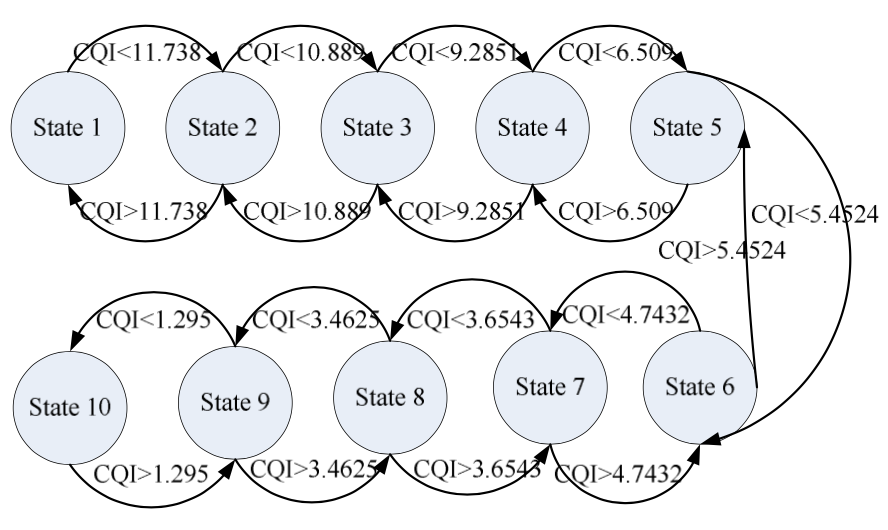
\includegraphics[width=0.7\linewidth]{figs/mtd}
	\caption {حالت‌های کیفیت در MTD و حدحساب هر یک}
	\label{fig:mtd}
\end{figure}

\begin{table}
	\begin{center}
		\caption{مقادیر تایمر مربوط به هر یک از حالات}
		\label{tbl:mtd}
		\begin{tabular}{|p{0.3\linewidth}|p{0.4\linewidth}|}
			\hline
			\textbf{پارامتر} & \textbf{DRX Inactivity Timer (TTI)}\\
			\hline
			حالت ۱ & $4$\\
			\hline
				حالت ۲ & $5$\\
			\hline
				حالت ۳ & $10$\\
			\hline
				حالت ۴ & $20$\\
			\hline
				حالت ۵ & $30$\\
			\hline
				حالت ۶ & $40$\\
			\hline
				حالت ۷ & $50$\\
			\hline
				حالت ۸ & $60$\\
			\hline
				حالت ۹ & $80$\\
			\hline
				حالت ۱۰ & $100$\\
			\hline
			\lr{\textbf{T\_trig}} & $6$\\
			\hline
		\end{tabular}
	\end{center}
\end{table}

\subsection{Optimized DRX/DTX}
راهکار ارائه شده در مقاله \cite{}، از بسیاری جهات از راهکار‌های ارائه شده در دو مقاله‌ی اول در زمینه استفاده از \lr{DRX/DTX} برای کاهش مصرف انرژی، بهینه‌تر است. در این مقاله، راهکار ارائه شده به این صورت است که ابتدا، بر اساس مدت زمان قابل‌قبول (بودجه زمانی) جریان‌\LTRfootnote{Flow}‌های داده مرتبط با یک گره، دوره‌ی کوتاه آن و سپس دوره‌ی بلند‌مدت آن را تعیین می‌نماید. سپس بر اساس پارمتر‌های تعیین شده، مقادیر \lr{On Duration} و \lr{Inactivity Timer} به‌ دست ‌می‌آید.

\subsubsection{تعیین زمان دوره}
در اولین گام از این راهکار، همان‌طور که گفته شد، به تعیین مقدار زمان دوره‌ی کوتاه (یا همان \lr{Short Cycle}) می‌پردازیم. بر این اساس، ابتدا باید اضطراری‌ترین جریان داده را مشخص نماییم. اضطراری‌ترین جریان داده، جریانی‌است که بودجه زمانی کمتری داشته و به عبارت دیگر انتظار می‌رود تا در زمان کمتری از جانب گره پاسخ یابد. این پارمتر را برای گره‌ی $i$ با نماد $D^{min}_i$ نمایش می‌دهیم. مدت زمان دوره‌ی کوتاه به وسیله‌ی فرمول \ref{eq:drx-short-cycle} محاسبه می‌شود.

\begin{equation}
T^S_i = \left\lfloor \frac{D^{min}_i}{T^S_{i-1}} \right\rfloor . T^S_{i-1}
\label{eq:drx-short-cycle}
\end{equation}

در فرمول بالا همان‌طور که مشاهده می‌شود، زمان به دست آمده از $D^{min}_i$ کوچکتر و یا مساوی با آن است. پس حتی امکان پاسخ‌دهی جریان داده‌ای با کمترین زمان قابل‌قبول را نیز ارضا می‌کند و هیچ جریان داده‌ای به واسطه طولانی بودن زمان دوره از دست نمی‌رود (\lr{Miss} نمی‌شود). حال، برای به دست آوردن مدت زمان دوره‌ی طولانی مدت، ابتدا در بین سرویس‌های مرتبط با گره، کوتاه‌ترین زمان پاسخگویی قابل‌قبول را یافته و بر اساس فرمول \ref{eq:drx-long-cycle}، محاسبه‌ی زمان دوره را انجام می‌دهیم. کوتاه‌ترین زمان پاسخگویی قابل‌قبول را برای گره $i$ با نماد $S^{min}_i$ نمایش می‌دهیم.

\begin{equation}
T^L_i = \left\lfloor \frac{S^{min}_i}{T^S_i} \right\rfloor . T^S_i
\label{eq:drx-long-cycle}
\end{equation}

همانطور که در فرمول فوق مشاهده می‌شود، مدت‌زمان دوره‌ی طولانی یک گره، در واقع ضریبی از مدت‌زمان دوره‌ی کوتاه آن می‌باشد. علاوه بر این، گزاره‌ی بالایی در مورد این فرمول نیز کاربرد دارد. یعنی به دلیل آن که $T^L_i$ کوچکتر و یا مساوی $S^{min}_i$ است، در نتیجه حتی کوتاه‌ترین زمان در میان زمان‌های قابل‌قبول برای پاسخ‌دهی به سرویس‌های مرتبط با گره را نیز ارضا خواهد کرد و به عبارت دیگر، سرویسی به دلیل طولانی بودن زمان دوره از دست نخواهد رفت.

\subsubsection{تعیین مدت‌زمان \lr{On Duration} و \lr{Inactivity Timer}}
برای محاسبه‌ی مدت‌زمان \lr{On Duration} راهکار ارائه شده به این صورت است که مجموع بیشینه‌ی حجم بسته‌ی جریان‌هایی را در نظر می‌گیریم که بودجه‌ی زمانی‌شان، برابر با مدت‌زمان دوره‌ی کوتاه که در مرحله‌ی قبل محاسبه کردیم باشد. سپس این مقدار را بر حداقل میزان کانال\LTRfootnote{Channel} گره‌ی مدنظر تقسیم می‌نماییم. لازم به ذکر است که مقدار از ضرب $\Omega$ که بیانگر تعداد بلوک‌های منبع\LTRfootnote{Resource Block (RB)} است در $C^{min}_i$ که بیانگر حداقل نرخ کانال\LTRfootnote{Channel Rate} بوده و واحد آن نیز (\lr{bits/RB}) می‌باشد، محاسبه می‌شود. علاوه بر این، همان‌طور که در فرمول \ref{eq:drx-on-duration} مشاهده می‌شود؛ یک مقدار حداقلی (در اینجا ۱) نیز برای محاسبه زمان \lr{On Duration} در نظر گرفته می‌شود.

\begin{equation}
O_i = \max \left\{ \left\lceil \frac{\Sigma_{D_j = T^S_i, \forall flow_j \in U E_i} Q^{max}_j}{C^{min}_i \times \Omega} \right\rceil , 1 \right\}
\label{eq:drx-on-duration}
\end{equation}

\par
دلیل چنین رویکردی این است که مطمئن باشیم حتی با کمترین منابع، در مدت زمان \lr{On Duration} قادر به دریافت تمام بسته‌های جریان داده هستیم.

\par
اما برای محاسبه \lr{Inactivity Timer}، ابتدا لازم است تا \lr{expected packet loss rate} را که آن را با نماد $E_{i, j}$ نمایش می‌دهیم، برای هر گره $i$ و هر جریان داده‌ای $j$ محاسبه کنیم. با فرض این که تعداد بسته‌های مربوط به یک جریان داده، $M_j$ عدد باشد و هر کدام از این بسته‌ها دارای تاخیری در بازه‌ی $1..D_j$ باشد، (اگر بیش از $D_j$ یا همان بودجه‌ی زمانی تاخیر داشته باشیم اصولا بسته از دست رفته است) مقدار $E_{i, j}$ از فرمول \ref{eq:drx-eij} محاسبه می‌شود.

\begin{equation}
E_{i, j} = \sum^{M_j}_{t_m = 1..D_j, m} Prob(t_m) \times Loss(m)
\label{eq:drx-eij}
\end{equation}

\begin{equation}
Loss(m) = \frac{M_j - \left(\Sigma_{m = 1..M_j}(\phi_m + \eta_m)\right)}{M_j}
\label{eq:drx-loss}
\end{equation}

\begin{equation}
\phi_m = 
\begin{cases}
	1, &$if$ \; X_m \leq D_j\\
	0, &$otherwise$
\end{cases}
\label{eq:drx-phi}
\end{equation}

\begin{equation}
\eta_m = 
\begin{cases}
	1, &$if$ \; X_m > D_j \; $and$ \; Y_m \leq \hat{\Gamma}^I_j \\
	0, &$otherwise$
\end{cases}
\label{eq:drx-eta}
\end{equation}

\par
تابع $Prob$ به صورت شهودی از سیستم به دست می‌آید و فرمول $Loss$ در \ref{eq:drx-loss} آمده است. برای محاسبه این تابع برای بسته‌ی $m$، به دو پارامتر نیاز است که این پارامترها به ترتیب $\phi_m$ و $\eta_m$ می‌باشند. پارامتر اول که در فرمول \ref{eq:drx-phi} آمده است، بیانگر این است که آیا بسته در زمان \lr{On Duration} گره قابل دریافت است یا خیر و پارامتر دوم که در فرمول \ref{eq:drx-eta} به آن اشاره گردیده است، بیانگر این امر است که آیا بسته در زمان  \lr{Inactivity Timer} قابل دریافت است یا خیر. مجموع این دو پارامتر اگر برابر با یک باشد به این معنی است که بسته از جانب گره قابل دریافت بوده است.  همان‌طور که مشاهده می‌شود، در فرمول \ref{eq:drx-loss} از مجموع این دو پارامتر استفاده گردیده است تا احتمال دریافت بسته سنجیده شود.

\par
پس از محاسبه‌ی تمامی $E_{i, j}$ها، برای هر جریان داده‌ی $j$ مقدار کمینه $E_{i, j}$ به عنوان مقدار کاندید \lr{Inactivity Timer} انتخاب می‌شود. لازم به ذکر است که دلیل انتخاب مقدار کمینه، این است که مقدار $P^{loss}_{i, j}$ (این پارامتر، بیانگر میزان قابل‌قبول \lr{Loss} شدن بسته‌های جریان $j$ در گره $i$ می‌باشد) ثابت بوده و در نتیجه تاثیری در \lr{Loss} شدن بسته‌ها ندارد؛ پس بدیهی است که کمترین مقدار \lr{Inactivity Timer}، به دلیل کمتر بیدار بودن گره، باعث کاهش مصرف انرژی می‌شود. سپس از بین تمامی کاندیدهای انتخاب شده، بیشترین مقدار به عنوان \lr{Inactivity Timer} گره موردنظر انتخاب می‌گردد. دلیل انتخاب مقدار بیشینه در این مرحله، این است که مقدار انتخاب شده به ازای تمامی جریان‌های داده قابل‌قبول باشد و به عبارت دیگر، مقدار نهایی \lr{Inactivity Timer} ،$P^{loss}_{i, j}$ مرتبط با همه‌ی جریان‌های داده گره را ارضا کند. 

\subsubsection{زمان‌بندی بسته‌ها}
علاوه بر استفاده از مکانیزم \lr{DRX/DTX} در مقاله‌ی مورد بررسی، یکی دیگر از ایده‌های مطرح شده در این مقاله، استفاده از یک مکانیزم ابداعی جهت زمان‌بندی بسته‌ها می‌باشد. در این مکانیزم بسته‌های مرتبط با هر گره، در یک صف در گره کنترل‌کننده نگه‌داری می‌شود. سپس گره‌کننده، بلوک منبعی را به هر یک از گره‌هایی که بسته‌ای جهت پردازش داشته باشند و زمان \lr{Inactivity Timer} آن‌ها رو به اتمام باشد؛ تخصیص می‌دهد. سپس بلوک‌های باقی‌مانده مابین گره‌های دیگر که اولویت پایین‌تری دارند تقسیم می‌شود. این عمل منجر به افزایش کیفیت سیستم شده و احتمال \lr{Loss} شدن بسته‌های داده‌ای جریان‌های گره را کاهش می‌دهد.

\section{راهکارهای مبتنی بر گراف}
در مقالاتی که در ادامه به بررسی آن‌ها خواهیم پرداخت، ایده‌ی اصلی مطرح شده، استفاده از گراف‌های درختی برای کاهش فواصل میان گره‌های شبکه می‌باشد. این کاهش فاصله منجر به کاهش مصرف انرژی به هنگام ارسال و دریافت اطلاعات میان گره‌ها می‌شود. در ادامه به بررسی راهکار مقاله‌ی اول از این دسته خواهیم پرداخت.

\subsection{درخت EGF}
در مقاله \cite{} راهکاری که ارائه شده، این است که محیط سیستم مبتنی بر اینترنت اشیا به لحاظ جغرافیایی به نواحی‌ای از محیط‌های محلی خوشه‌بندی شود که در هر یک از آن‌ها یک گره به عنوان گره سرگروه فعالیت می‌کند. وظیفه‌ی گره سرگروه این است که ارتباط لازم میان گره هدف و \lr{Base Station} را برقرار نماید. به این وسیله مصرف انرژی شبکه مبتنی بر اینترنت اشیا کاهش چشمگیری می‌یابد. زیرا در هنگام برقراری ارتباط، نیازی به روشن بودن مدار ارتباطی همه گره‌ها نیست و نکته‌ی اصلی همین است که بخش زیادی از انرژی مصرف شده توسط گره‌ها مربوط به مدار ارتباطی آن‌ها می باشد.

\subsubsection{مدل انرژی}
در مقاله‌ی مذکور برای مدل‌سازی ریاضی انرژی از توابع زیر استفاده شده است. لازم به ذکر است که فرمول \ref{eq:egf-etx} بیانگر میزان انرژی لازم برای ارسال $k$ بیت پیام به فاصله‌ی $d$، فرمول \ref{eq:egf-erx} بیانگر میزان انرژی مصرفی جهت دریافت $k$ بیت پیام و فرمول \ref{eq:egf-energy} بیانگر میزان انرژی لازم برای انتقال (ارسال و دریافت) $k$ بیت پیام به فاصله $d$ می‌باشد.

\begin{equation}
E_{tx} = a \times k + b \times k \times d^n_{ij}
\label{eq:egf-etx}
\end{equation}

\begin{equation}
E_{rx} = c \times k
\label{eq:egf-erx}
\end{equation}

\begin{equation}
C_{ij}(K) = 
\begin{cases}
	a \times k + b \times k \times d^n_{ij} & $if$ \; j \; $is$ \; BS\\
	E_{tx} + E_{rx} & $otherwise$
\end{cases}
\label{eq:egf-energy}
\end{equation}

\par
همان‌گونه که در فرمول‌های بالا ملاحظه ‌می‌شود؛ $a$، $b$ و $c$ ثابت هستند  و $d_{ij}$ بیانگر فاصله‌ي میان دو گره $i$ و $j$ است. علاوه بر این، این نکته از فرمول‌های بالا برداشت می‌شود که دریافت پیام توسط $BS$ یا همان \lr{Base Station} محدودیتی ندارد و به همین دلیل در مدل ریاضی مقاله‌ی تحت بررسی از این مقدار چشم‌پوشی شده است.

\begin{figure}
	\centering
	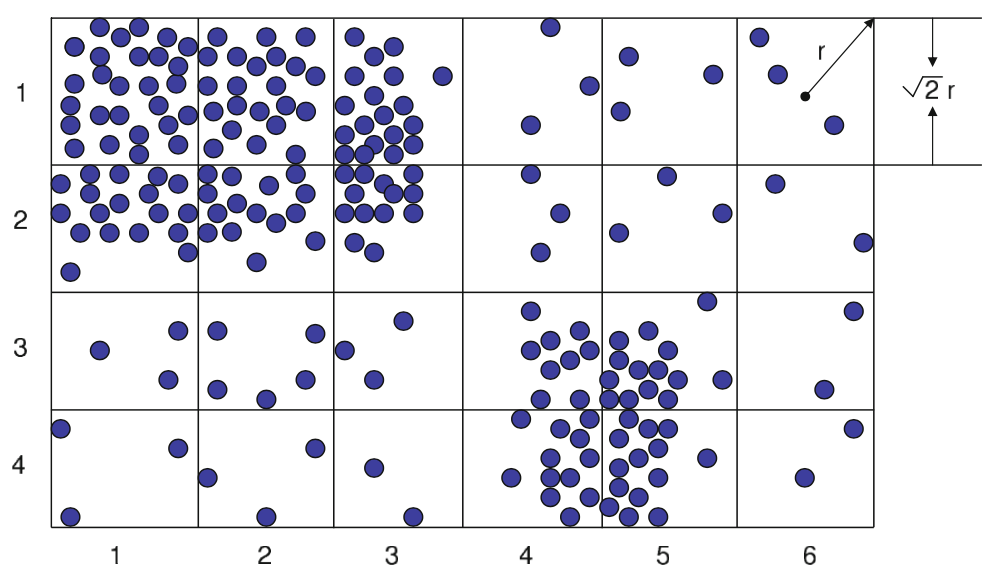
\includegraphics[width=0.7\linewidth]{figs/egf-env}
	\caption {محیط مورد بررسی در مقاله‌ی \cite{}}
	\label{fig:egf-env}
\end{figure}

\subsubsection{ساخت درخت EFG}
فرض کنید محیطی که قرار است درخت را در آن تشکیل دهیم، محیط نمایش داده شده در شکل \ref{fig:egf-env} است. برای ساخت درخت، همانطور که در الگوریتم شکل \ref{fig:egf-al1} دیده می‌شود، ابتدا محیط را به سلول\LTRfootnote{Cell}های مربعی با طول ضلع $\sqrt{2}r$ (که $r$ بیانگر شعاع ارتباطی حسگرها است و در این مقاله برای تمامی حسگرها یکسان است) تقسیم‌بندی می‌نماییم.
\par
پس از آن که تقسیم‌بندی سلول‌ها انجام گردید؛ در الگوریتم ارائه شده، نوبت به مرحله‌ی محاسبه‌ی وزن می‌رسد. در این مرحله، به ازای هر گره، وزن میان این گره و گره‌های مجاور آن (یعنی گره‌های بالا، پایین، چپ و راست گره مورد نظر) به کمک الگوریتم دوم که در شکل \ref{fig:egf-al2} مشهود است؛‌ محاسبه می‌شود. در ادامه به توضیح این الگوریتم خواهیم پرداخت.
\par
اما بعد از آن که محاسبه‌ی وزن میان سلول‌های محیط صورت گرفت؛ ابتدا تمامی سلول‌ها را به عنوان یک زیرمحیط\LTRfootnote{Sub-Region} در نظر می‌گیریم و وزن میان هر جفت از این زیرمحیط‌ها را به صورت نزولی مرتب می‌نماییم. در این مرحله، هر بار؛ دو زیرمحیط که بین‌شان بالاترین وزن موجود است با یکدیگر ادغام کرده و یک زیرمحیط جدید ایجاد می‌کنیم که در واقع والد دو زیرمحیط قبلی است. بدین صورت گره‌های دو زیرمحیط قبلی به عنوان گره‌های فرزند\LTRfootnote{Child Nodes} زیرمحیط جدید معرفی می‌شوند.
\par
پس از آنکه زیرمحیط جدید تعریف شد، در واقع همان مرحله‌ی قبلی - که محاسبه وزن بود - باید برای آن صورت گیرد. اما با این تفاوت که این بار، وزن باید برای یک زیرمحیط محاسبه شود و نه یک سلول که روش محاسبه‌ی وزن برای زیرمحیط در الگوریتم شکل \ref{fig:egf-al3} آمده است. در مورد این الگوریتم نیز جلوتر به تفصیل صحبت می‌نماییم. سپس، با محاسبه‌ی وزن زیرمحیط‌های مجاور زیرمحیط مدنظر (زیرمحیط‌های بالا، پایین، چپ و راست آن) کار الگوریتم در گام اول به پایان می‌رسد و عملیات ذکر شده در دو پاراگراف اخیر (خط‌های ۱۰ الی ۱۷ شبه کد الگوریتم شکل \ref{fig:egf-al1}) تکرار می‌گردد. این عملیات تا آن‌جایی ادامه پیدا ‌می‌کند که دیگر فقط یک زیرمحیط در تمام محیط تحت پوشش سیستم باقی بماند.
به این صورت گراف محیط شکل \ref{fig:egf-env} ساخته شده و در شکل \ref{fig:egf-graph} قابل مشاهده است. لازم به ذکر است که در گراف درختی ساخته شده، سلول‌ها در موقعیت برگ‌های درخت قرار می‌گیرند.

\begin{figure}
	\centering
	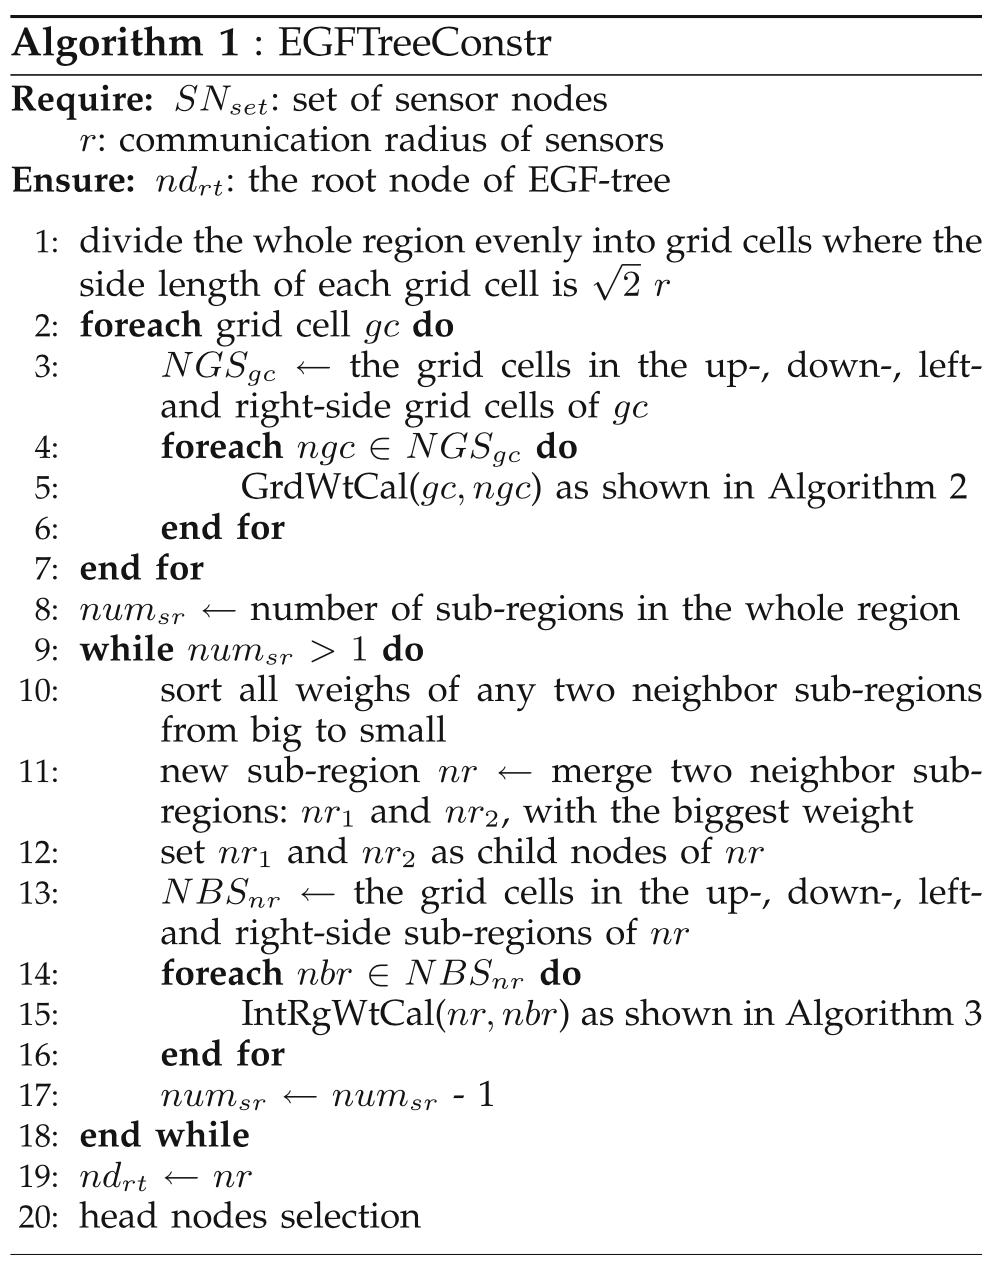
\includegraphics[width=0.7\linewidth]{figs/egf-al1}
	\caption {شبه کد الگوریتم ساخت درخت EGF}
	\label{fig:egf-al1}
\end{figure}

\begin{figure}
	\centering
	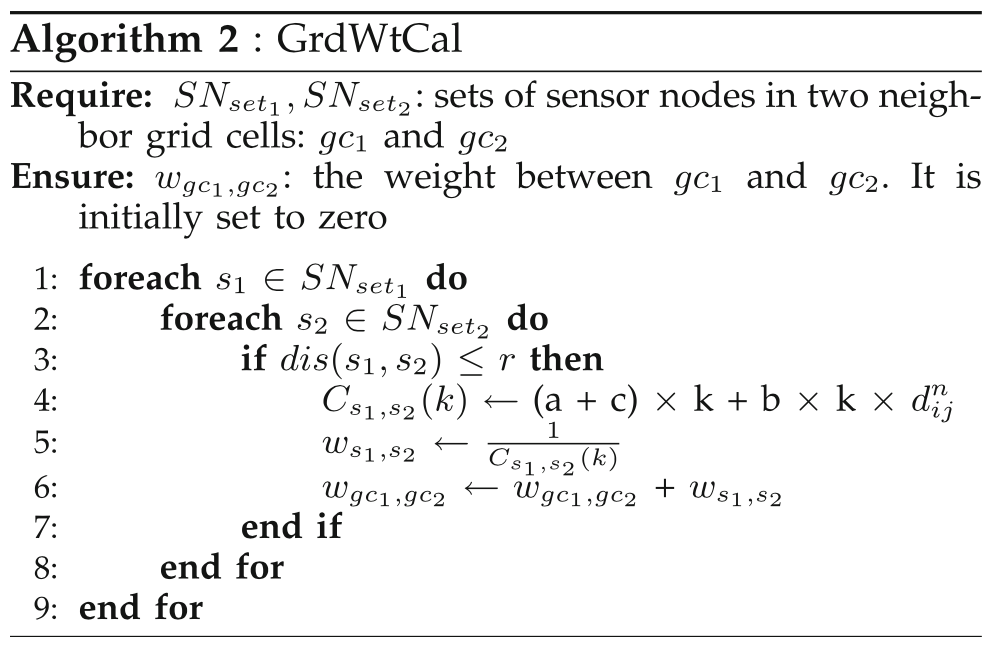
\includegraphics[width=0.7\linewidth]{figs/egf-al2}
	\caption {شبه کد الگوریتم محاسبه‌ی وزن میان سلول‌ها}
	\label{fig:egf-al2}
\end{figure}

\begin{figure}
	\centering
	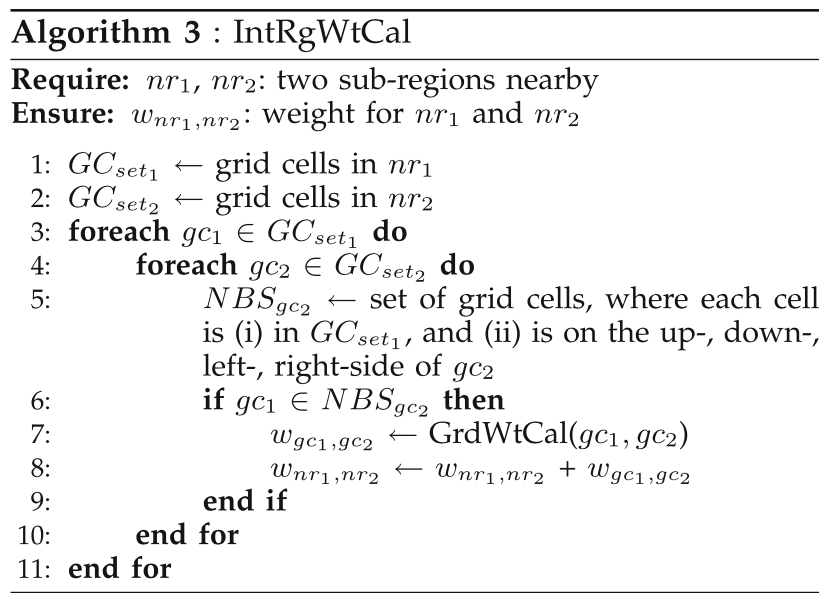
\includegraphics[width=0.7\linewidth]{figs/egf-al3}
	\caption {شبه کد الگوریتم محاسبه‌ی وزن میان زیرمحیط‌ها}
	\label{fig:egf-al3}
\end{figure}

\begin{figure}
	\centering
	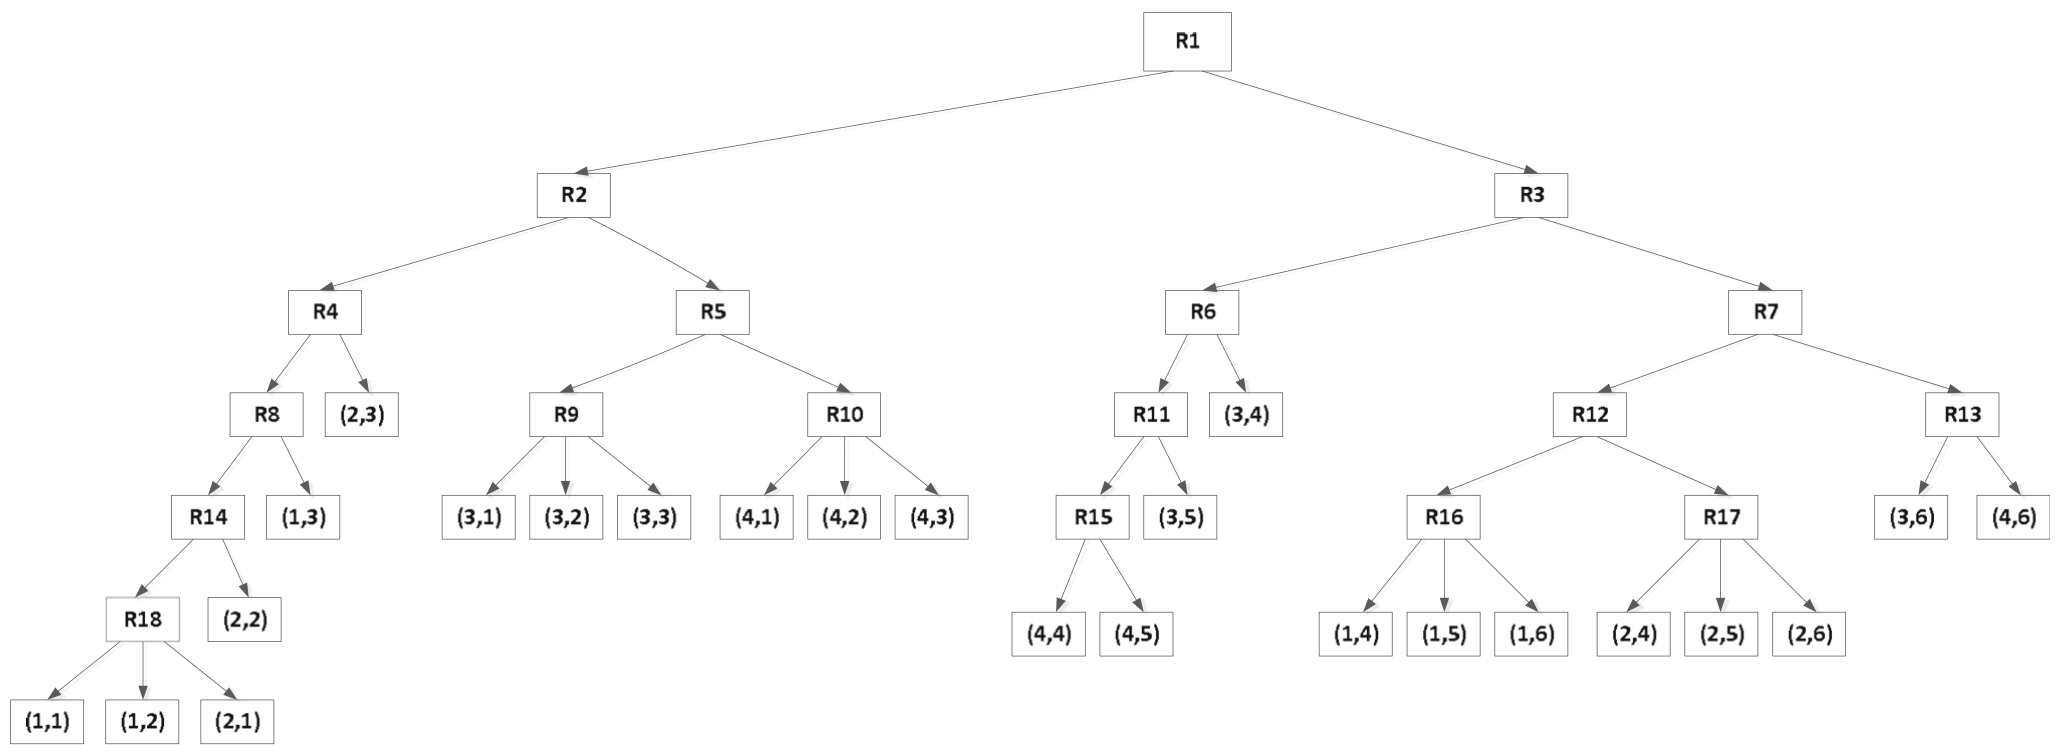
\includegraphics[width=0.7\paperheight,angle=90,origin=c]{figs/egf-graph}
	\caption {گراف حاصل شده برای محیط شکل \ref{fig:egf-env}}
	\label{fig:egf-graph}
\end{figure}

\par
در الگوریتم شکل \ref{fig:egf-al2} برای محاسبه‌ی وزن میان دو سلول مجاور، به ازای هر جفت گره‌ای از سلول اول و سلول دوم (یعنی گره اول در جفت گره موردنظر، متعلق به سلول اول و گره دوم متعلق به سلول دوم باشد) عملیات زیر را انجام می‌دهیم. ابتدا، بررسی انجام می‌شود که فاصله‌ی دو گره از هم بیشتر از شعاع ارتباطی (یا همان $r$) نباشد. سپس در صورتی که فاصله‌ی بین دو گره، کمتر و یا مساوی شعاع ارتباطی‌شان بود؛ وزن میان آن دو گره از معکوس $C_{ij}(k)$  که محاسبه‌ی آن در فرمول \ref{eq:egf-energy} شرح داده شد به دست ‌می‌آید. سپس از مجموع وزن‌های به دست آمده در میان گره‌ها، وزن کلی میان دو سلول حاصل می‌گردد. در فرمول \ref{eq:egf-weight} می‌توانید نمونه محاسبه وزن میان دو سلول قابل مشاهده در شکل \ref{fig:egf-weight} را بررسی نمایید.

\begin{equation}
w_{(3,1),(3,2)} = \frac{1}{C_{S_2,S_4}(k)} + \frac{1}{C_{S_2,S_5}(k)} + \frac{1}{C_{S_3,S_4}(k)}
\label{eq:egf-weight}
\end{equation}

\begin{figure}
	\centering
	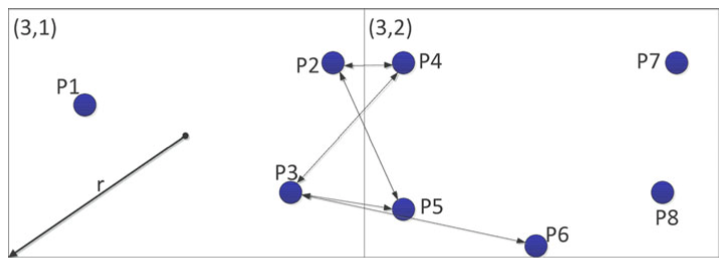
\includegraphics[width=0.7\linewidth]{figs/egf-weight}
	\caption {محاسبه‌ی وزن میان دو سلول مجاور}
	\label{fig:egf-weight}
\end{figure}

\par
از فرمول بالا می‌توان دریافت که فاصله‌ی دو گره با وزن آن نسبت عکس دارد. یعنی هر آن چه فاصله‌ی میان گره‌ها بیشتر باشد، انرژی مصرفی بیشتری مورد نیاز است و همین باعث کاهش وزن رابطه‌ی میان آن دو گره در گراف می‌شود.

\par
اما برای محاسبه‌ی وزن میان دو زیرمحیط، همان‌گونه که در الگوریتم شکل \ref{fig:egf-al3} مشاهده می‌شود، به این صورت است که برای هر سلول در زیرمحیط دوم، سلول‌هایی را می‌یابیم که اولا؛ عضو زیرمحیط اول باشند و دوما؛ با سلول مدنظر مجاورت داشته باشند. سپس باقی مراحل همانند محاسبه وزن برای سلول‌ها خواهد بود. بدین ترتیب که به ازای هر جفت سلولی که با یکدیگر، رابطه‌ی مذکور را داشتند وزن را محاسبه می‌کنیم و از مجموع اوزان به دست آمده، وزن کلی مابین دو زیرمحیط حاصل می‌گردد.

\subsubsection{تجمیع کوئری‌ها}
یکی از راهکارهای ارائه شده‌ی دیگر در این مقاله، تجمیع کوئری‌ها است. تجمیع کوئری‌ها باعث می‌شود تا درخواست ارسالی به حسگرها از طریق یک رابط منتقل گردد و سپس در برگشت اطلاعات نیز تمامی حسگر‌ها، اطلاعات خود را به یک گره سرگروه ارسال کرده و ادغام این اطلاعات با یکدیگر در گره سرگروه انجام شده و نتیجه فقط از طریق از طریق ارتباط آن گره با \lr{Base Station} بازگردانی شود. برای این کار، لازم است ابتدا مدل کوئری ارائه شده را تعریف نماییم.

\begin{equation}
Q = \langle ID, R, T, A, F \rangle
\label{eq:eqf-query-model}
\end{equation}

در فرمول \ref{eq:eqf-query-model} مدل کوئری‌های ارائه شده قابل مشاهده است. در این مدل، $ID$، بیانگر شناسه کوئری، $R$ بیانگر محیط مرتبط با کوئری، $T$ مشخص کننده‌ی مدت زمان کوئری، $A$ بیانگر مشخصه‌ها و پارامترهای ارسالی کوئری و $F$ بیانگر تناوب کوئری می‌باشد. نکته‌ی مهم این است که هر کوئری در واقع متشکل از چندین زیرکوئری\LTRfootnote{Sub-Query} می‌باشد که در پارامتر‌های کوئری به غیر از $Q$ یکسانند و به عبارت دیگر، هر زیرکوئری، بیانگر یک کوئری مرتبط با یکی از زیرمحیط‌های موردنیاز کوئری اصلی می‌باشد. در فرمول \ref{eq:eqf-query-agg} این مسئله به خوبی مشهود است.

\begin{equation}
Q = \langle R, T, A, F \rangle = \langle R_1, T, A, F \rangle + \langle R_2, T, A, F \rangle + \ldots + \langle R_j, T, A, F \rangle
\label{eq:eqf-query-agg}
\end{equation}

حال که به مفهوم زیرکوئری پرداختیم؛ می‌توان تجمیع زیرکوئری‌هارا تشریح کرد. برای تجمیع زیرکوئری‌ها، دو وضعیت مطرح شده است. به این صورت که یا یک زیرکوئری به لحاظ محیط ($R$)، زیرمجموعه‌ی دیگری باشد. و یا دو زیرکوئری به لحاظ محیط‌شان دارای اشتراک باشند به طوری که رابطه‌ی
 $S_{R_i \cap R_j}/S_{R_i \cup R_j} \geq \alpha$ 
 برقرار باشد. ($\alpha$ یک ثابت است که مقدار آن در بازه $0..1$ می‌باشد.)
\par
نحوه‌ی تجمیع زیرکوئری‌ها را در وضعیت اول و دوم که در بالا ذکر شده است، به ترتیب در فرمول‌های \ref{eq:eqf-query-subsume} و \ref{eq:eqf-query-intersect} آمده است. لازم به ذکر است که در فرمول \ref{eq:eqf-query-subsume}، 
$R_i \subseteq R_j$
 و در فرمول \ref{eq:eqf-query-intersect}، 
$R_{ij} = R_i \cap R_j$ می‌باشد.

\begin{equation}
Q_{i+j} = 
\begin{cases}
	\langle R_j, \{T_i, T_j\}, A_i, F_i \rangle & $if$ \; A_i = A_j \; $and$ \;F_i = F_j \\
	\langle R_j, T_i, \{A_i, A_j\}, F_i \rangle & $if$ \; T_i = T_j \; $and$ \;F_i = F_j
\end{cases}
\label{eq:eqf-query-subsume}
\end{equation}

\begin{equation}
Q_{i+j} = 
\begin{cases}
	\langle R_{ij}, \{T_i, T_j\}, A_i, F_i \rangle & $if$ \; A_i = A_j \; $and$ \;F_i = F_j \\
	\langle R_{ij}, T_i, \{A_i, A_j\}, F_i \rangle & $if$ \; T_i = T_j \; $and$ \;F_i = F_j
\end{cases}
\label{eq:eqf-query-intersect}
\end{equation}

\par
تا این جا  با سازوکار تجمیع داده‌ها کوئری‌ها آشنا شدیم. در مرحله بازگشت داده‌ها در پاسخ به کوئری نیز همین شرایط مطرح است. برای مثال، در شکل \ref{fig:egf-agg} می‌بینیم که $GH5$ به عنوان گره سرگروه انتخاب می‌شود و داده‌های به دست یافته از سلول‌های $(3,2)$ و $(4,2)$، به وسیله‌ی سرگروه‌هایشان (یعنی $GH6$ و $GH9$) و از طریق گره $P5$ به $GH5$ انتقال می‌یابد. داده‌های به دست آمده از این سه حسگر، در خود $GH5$ تجمیع می‌شود و چون داده‌ی دیگری برای تجمیع با داده‌های فعلی وجود ندارد، نیازی به سطح بالاتری از گره‌ها نداریم. در نهایت داده‌های تجمیع شده در $GH5$ از طریق گره $P1$ به \lr{Base Station} بازگردانده می‌شوند.

\begin{figure}
	\centering
	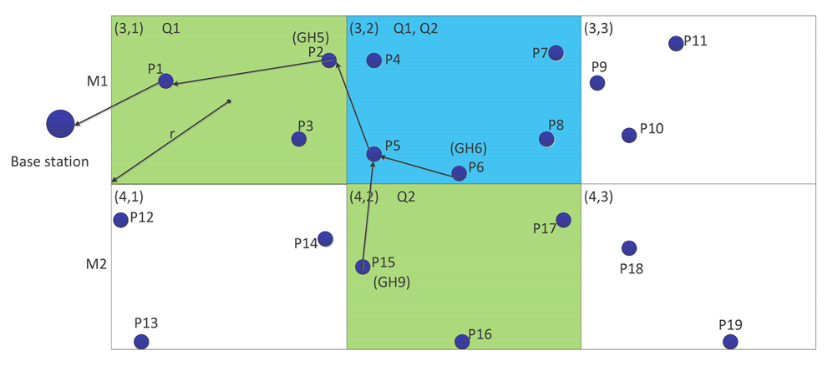
\includegraphics[width=0.7\linewidth]{figs/egf-agg}
	\caption {بازگرداندن داده به \lr{Base Station}}
	\label{fig:egf-agg}
\end{figure}

\par
علاوه بر این، در این مقاله برای تعیین گره‌ی سرگروه هر زیرمحیط از الگوریتم \lr{LEACH} استفاده شده است که با تغییر مداوم سرگروه‌ها از کاهش چشم‌گیر یک گره خاص جلوگیری نموده و منجر به افزایش طول عمر سیستم می‌گردد.

\subsection{درخت ECH}
از بسیاری جهات، رویکرد مقاله \cite{} همانند مقاله‌ی قبلی است. هر دو از رویکرد تجمیع کوئری یکسانی استفاده کرده‌اند، هر دو مدل‌های انرژی و کوئری‌شان یکسان است و هر دو اساس کارشان ساختن درخت برای توپولوژی شبکه مبتنی بر اینترنت اشیا می‌باشد. اما تفاوت عمده این دو رویکرد در نحوه ساخت درختشان است که عملکردشان را متفاوت می‌سازد.

\par
در الگوریتم ارائه شده توسط این مقاله که در شکل \ref{fig:ech-al1} دیده می‌شود، همانند مقاله پیشین، ابتدا محیط به سلول‌های با ضلع $\sqrt{2}r$ تقسیم می‌گردد. سپس سلول‌های تقسیم‌بندی شده، هر یک به عنوان یک زیرمحیط در نظر گرفته می‌شوند و الگوریتم شکل \ref{fig:ech-al2} بر روی آن‌ها اعمال می‌گردد. می‌توان گفت که اساس کار این مقاله، در واقع همین الگوریتم است و تفاوت اصلی رویکرد این مقاله با مقاله‌ی پیشین در همین مرحله رقم می‌خورد. در راهکار ارائه شده در این مقاله، دو عدد ثابت به عنوان حداقل و حداکثر تعداد گره‌های فرزند (و یا در سطوح بالاتر: زیرمحیط‌ها) در یک زیرمحیط در نظر گرفته شده است که به ترتیب، با $m$ و $M$ نمایش داده می‌شوند. الگوریتم شکل \ref{fig:ech-al2} بیان می‌دارد که ابتدا تعداد گره‌های فرزند بررسی می‌شود. اگر تعداد گره‌ها در بازه‌ی $m..M$ بود، همان گره‌ها به عنوان یک زیرمحیط با سطح بالاتر به عنوان خروجی الگوریتم برگردانده می‌شود. اما اگر چنین نبود و تعداد بیش از $M$ باشد؛ تعداد $k$ گره از میان گره‌های فرزند انتخاب می‌شود. لازم به ذکر است که چون تعداد گره‌ها برابر با $num$ و تعداد حداقل و حداکثر فرزندان به ترتیب، برابر با $m$ و $M$ می‌باشد؛ پس مقدار $k$ باید در بازه $num/M..num/m$ قرار داشته باشد.
\par
پس از آن که این انتخاب در بین گره‌های فرزند صورت گرفت. برای هر گره باقی‌مانده وزن آن نسبت به $k$ گره انتخاب شده سنجیده می‌شود و در این بین هر کدام که وزن بیشتری را به عنوان حاصل، به دست آورد؛ آن گره فرزند گره مذکور از بین $k$ گره انتخابی می‌شود و اگر تعداد زیرگره‌ها برای یک گره بیش از $M$ شود. همین الگوریتم روی آن گره مخصوص مجددا اعمال می‌گردد. لازم به ذکر است که الگوریتم محاسبه‌ی وزن دقیقا همانند الگوریتم‌های شکل \ref{fig:egf-al2} و
\ref{fig:egf-al3}
 بوده و این عملیات تا زمانی ادامه می‌یابد که تعداد زیرمحیط‌ها از $m$ بیشتر باشد. به این ترتیب، زمانی که تعداد گره‌ها کمتر از $m$ شد؛ ریشه‌ی درخت مشخص شده و عملیات ساخت درخت پایان می‌یابد.

\par
در پایان می‌توانید درخت ساخته شده توسط الگوریتم ابداعی این مقاله را در شکل \ref{fig:ech-graph} مشاهده نمایید. همان‌گونه که در مقایسه‌ی این درخت با درخت شکل \ref{fig:egf-graph} مشهود است؛ وجه مشابهت هر دو درخت در این است که در هر دوی آن‌ها، سلول‌های تقسیم‌بندی شده‌ی محیط برگ‌های درخت می‌باشند. اما عمده تفاوت این دو درخت این است که درخت به دست آمده از الگوریتم مقاله‌ی \cite{}، درختی متوازن است و عمق کمتری دارد. همین امر می‌تواند سبب کاهش مسیر ارتباطی داده‌ها و درخواست‌ها گردیده و در نتیجه، میزان انرژی مصرفی سیستم‌های مبتنی بر اینترنت اشیا را کاهش دهد.

\begin{figure}
	\centering
	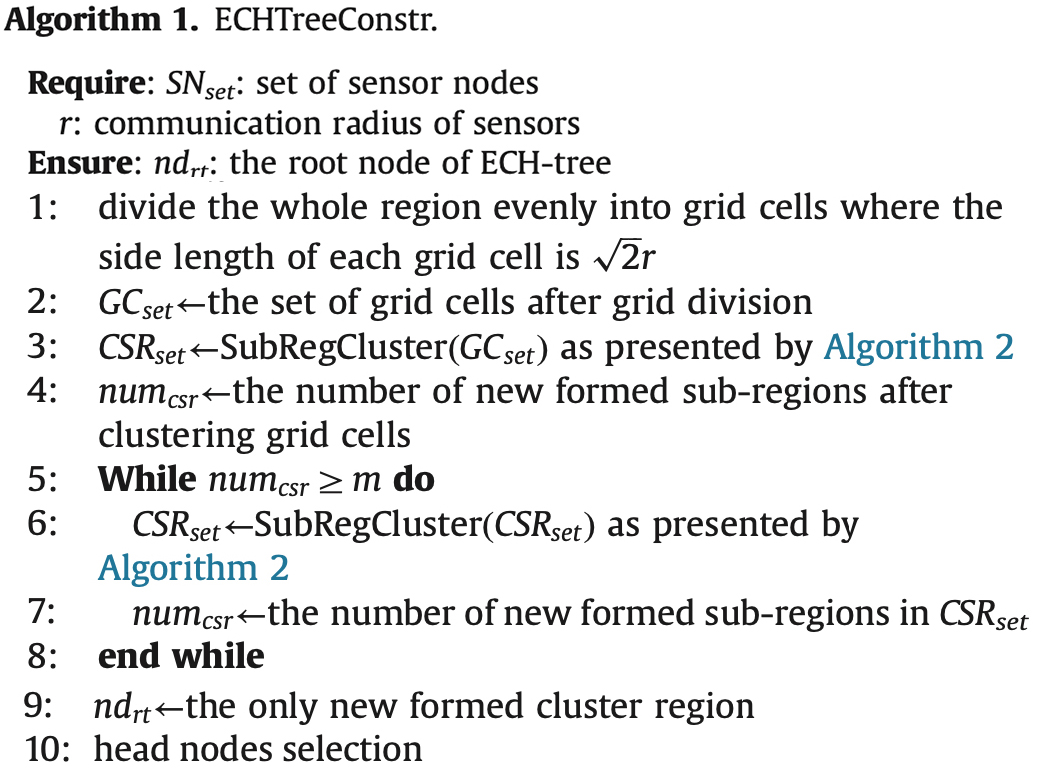
\includegraphics[width=0.7\linewidth]{figs/ech-al1}
	\caption {شبه کد الگوریتم ساخت درخت ECH}
	\label{fig:ech-al1}
\end{figure}

\begin{figure}
	\centering
	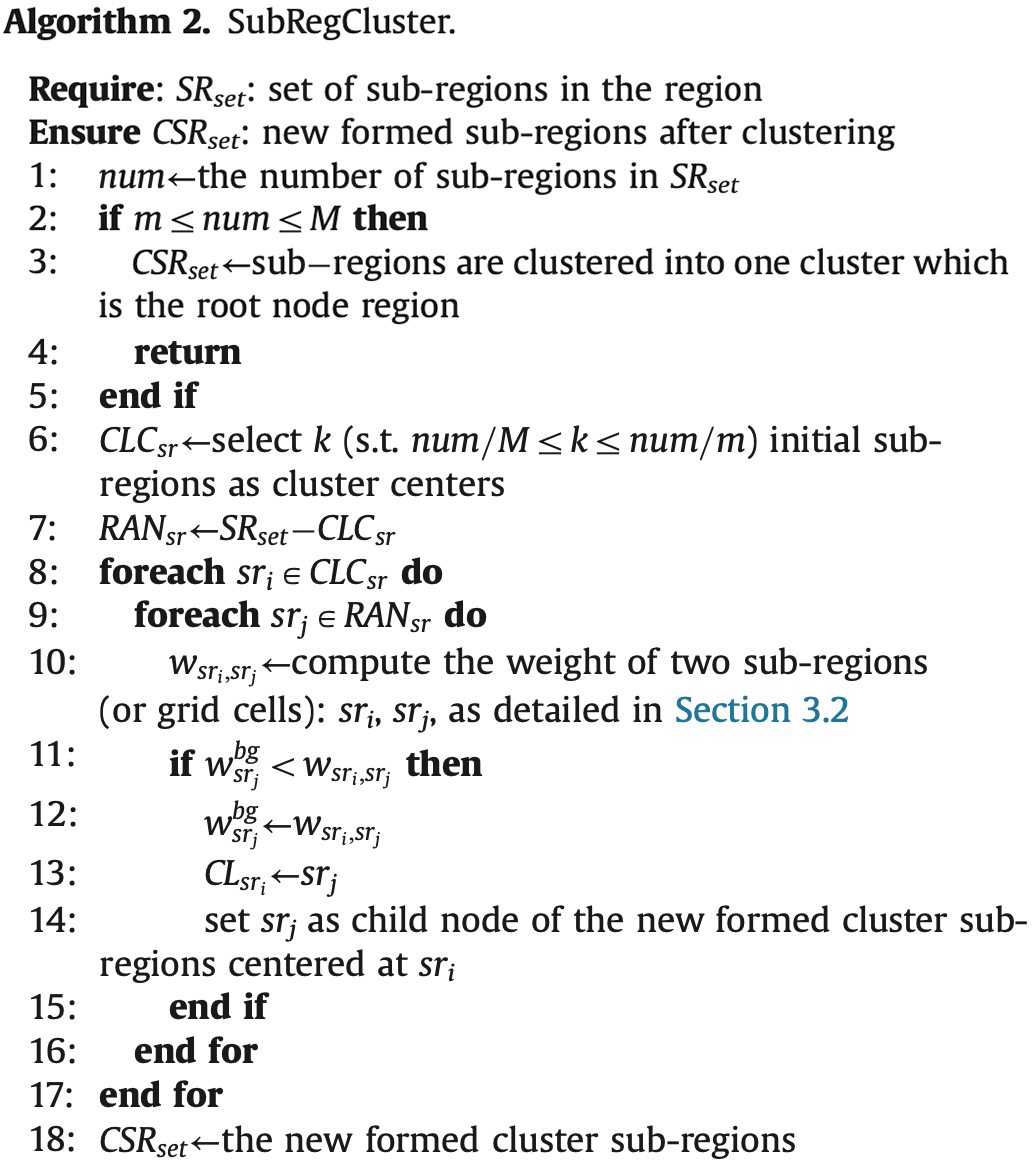
\includegraphics[width=0.7\linewidth]{figs/ech-al2}
	\caption {شبه کد الگوریتم خوشه‌بندی ECH}
	\label{fig:ech-al2}
\end{figure}

\begin{figure}
	\centering
	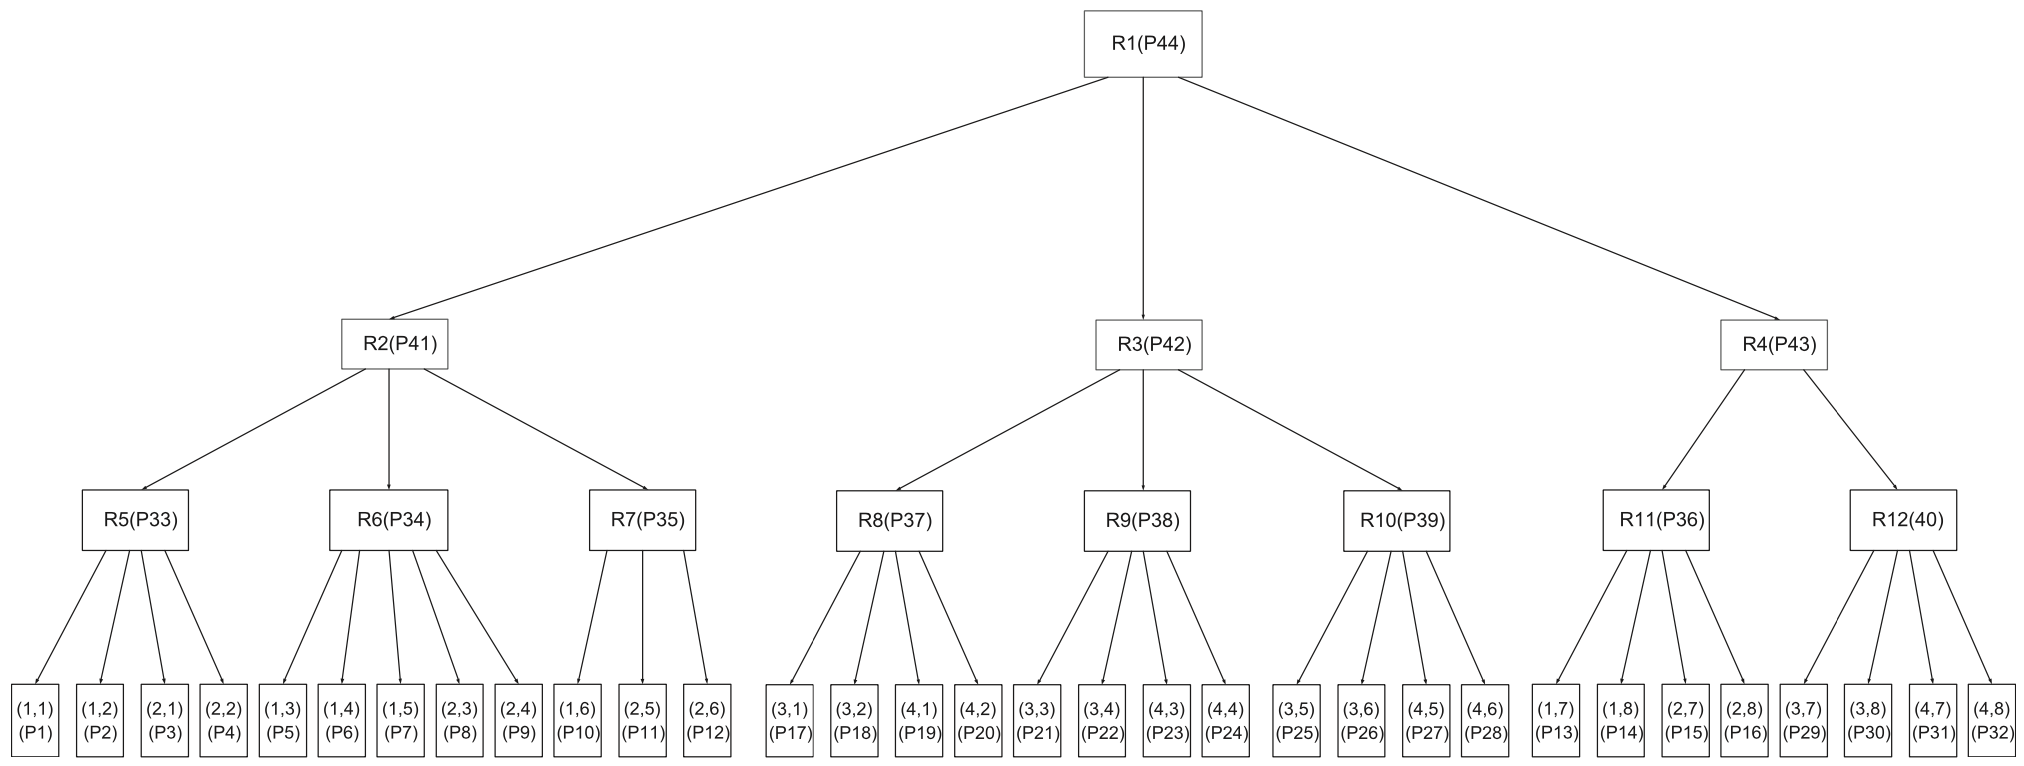
\includegraphics[width=0.7\paperheight,angle=90,origin=c]{figs/ech-graph}
	\caption {گراف ساخته شده با الگوریتم ECH}
	\label{fig:ech-graph}
\end{figure}

\section{راهکار \lr{Object Group Mobility} \lr{(OGM)}}
در راهکار ارائه شده در مقاله‌ی \cite{}، که با نام \lr{Object Group Mobility} معرفی شده است؛ شبکه‌ای از گره‌ها در نظر گرفته شده که می‌توانند در حرکت باشند (موقعیت‌شان را تغییر دهند) و همچنین در محیط مورد بررسی می‌تواند گروه‌های گوناگونی از گره‌ها وجود داشته باشد که فناوری ارتباطی آن‌ها با یکدیگر یکسان نیست. برای مثال در یک گروه ممکن است فناوری ارتباطی \lr{IEEE 802.15.4} به کار رود. در صورتی که در گروهی دیگر از \lr{RFID} و یا \lr{Bluetooth} استفاده می‌شود. پس به همین دلیل می‌توان گفت شبکه‌ی مورد بررسی و به تبع آن، راهکار ارائه شده دارای انعطاف بیشتری است.
\par
در این مقاله، فرض شده که محیط مورد بررسی $A$ متشکل از مجموعه ای از محیط‌های کوچک‌تر است که به آن‌ها \lr{Ambience} گفته می‌شود. ما برای سادگی و یکپارچگی اصطلاحات به‌کار رفته تا بدین جا، از همان لفظ زیرمحیط برای بیان این مفهوم استفاده می‌نماییم. پس محیط $A$ به شکل $A = \{a_1, a_2, \ldots, a_M\}$ قابل بیان است که $a_i$ بیان‌گر زیرمحیط $i$ام می‌باشد.
\par
سیستم ابداعی این مقاله، در واقع متشکل گروه‌هایی است که خود، مجموعه‌ای از \lr{Access Point (AP)}‌های ناهمگن هستند و می‌توانند در کنار یکدیگر کار کنند.  برای مثال اگر سیستم مورد بحث ما یک ساختمان هوشمند باشد، هر یک از واحد‌های آن یک گروه در سیستم ماست. هر یک از \lr{AP}های یک گروه، دارای فناوری ارتباطی مخصوص خودش است که با $\psi(AP)$ نمایش داده می‌شود. علاوه بر این، هر \lr{AP} تعدادی از زیرمحیط‌ها را پوشش می‌دهد که مجموعه‌ی زیرمحیط‌های تحت پوشش آن را با $C(AP)$ نمایش می‌دهند. بدیهی است  که هر حسگر فقط می‌تواند به \lr{AP}هایی وصل شود که فناوری ارتباطی یکسانی با آن داشته باشند.
\par
در راهکار ارائه شده، یک \lr{Content Server (CS)} به کنترل موقعیت حسگر‌ها می‌پردازد و علاوه بر این، هر حسگر دارای یک \lr{Home Network} 
($HN(n)$)
 است که در آن یک \lr{Agent} (که در مقاله با نام \lr{Home Agent} معرفی شده است) مسئول نگه‌داری اطلاعات مربوط به موقعیت حسگر است. برای این‌که به سازوکار ابداعی این مقاله آشنا شویم؛ فرض کنید یک گروه از گره‌ها را در اختیار داریم که آن‌ها را با $n_0, \ldots, n_m$ نمایش می‌دهیم. فرض می‌نماییم که در این گروه، گره $n_0$ به عنوان گره سرگروه انتخاب شده است. هر گره پیرو\LTRfootnote{Slave}، آدرسی که سرگروه به آن نسبت می‌دهد به عنوان \lr{Care-of-Address} خود ($CoA(n_i)$) معرفی می‌نماید. این آدرس در واقع همان $HN(n_0)$ است. بدین ترتیب زمانی که یک گره بخواهد با یکی از گره‌های $n_1, \ldots, n_m$ ارتباط برقرار کند، درخواست خود را (که می‌تواند شامل داده‌های مورد انتقالی و یا ... باشد) به $CoA(n_i)$ ارسال می‌نماید. سپس براساس $CoA(n_i)$ گره مقصد، درخواست به $HN(n_0)$ منتقل\LTRfootnote{Forward} می‌گردد و از آن‌جا توسط $n_0$ برای گره موردنظر ارسال می‌شود.

\par
از راهکار ارائه شده در بالا چنین بر می‌آید که اگر یک گره بخواهد موقعیت خود را تغییر دهد نیازمند به‌روزرسانی تمامی گره‌های پیروی دیگر نبوده و فقط کافیست اطلاعات موجود در $HN$ گره سرگروه به روزرسانی شود. بدیهی است که همین امر سبب کاهش داده‌های انتقالی و در نتیجه کاهش مصرف انرژی در سیستم‌های مبتنی بر اینترنت اشیا می‌گردد.

\par
پس از آنکه جابجایی یک گره در شبکه به وقوع پیوست، گره مذکور اطلاعات خود را از قبیل \lr{IPv6}، 
\lr{MAC Address}،
فناوری ارتباطی ($\psi(n)$)
و در صورتی که گره سرگروه باشد آدرسی که باید برای گره‌های پیرو \lr{Set} شود را به \lr{Content Server} ارسال می‌نماید. \lr{Content Server} دو وظیفه‌ی اصلی بعد از دریافت این اطلاعات از جانب یک گره دارد.

\begin{itemize}
\item{
به‌روزرسانی اطلاعات موقعیت و گروه‌ها: در این مرحله، \lr{CS} بعد از بررسی سازگاری گره اضافه شده به گروه، به‌روزرسانی اطلاعات را انجام می‌دهد. علاوه بر این در همین حین، \lr{CS} بررسی می‌کند که آیا امکان ادغام گروه موردنظر با سایر گروه‌ها وجود دارد یا خیر. به طور کلی، گروهی که گره $n$ در آن قرار دارد 
($\Gamma(n)$)
 اگر یکی از دو شرط مطرح شده را داشته باشد می‌تواند با گروه $\Gamma_i$ ادغام گردد. شرایط بدین شرح است که یا تمام گره‌هایی با فناوری ارتباطی مشابه، اخیرا گروه $\Gamma_i$ را ترک و به گروه $\Gamma(n)$ پیوسته باشند. و یا این که در گروه $\Gamma_i$ دیگر گره‌ای با فناوری ارتباطی مشابه وجود نداشته باشد.
}
\item{
تخمین موقعیت جغرافیایی حسگرها: بر اساس اطلاعات موقعیتی که به \lr{CS} ارسال شده است، \lr{CS} می‌تواند تخمینی در ارتباط با موقعیت جغرافیایی این حسگر داشته باشد. برای مثال اگر گره $n$ به گروه جدیدی بپیوندد؛ به ازای هر گره موجود در گروه جدید ($z$) می‌توان رابطه $\Phi(z) = C(AP(z)$ را معرفی کرد که بیانگر زیرمحیط‌هایی است که گره $z$ آن‌ها را پوشش می‌دهد. در نتیجه بدیهی است که این حسگرها در محیط اشتراکی به دست آمده، یعنی $\bigcap_{z \in \Gamma(n)} \Phi(z)$ قرار دارند. 
}
\end{itemize}

\par
در شکل \ref{fig:ogm-proc} می‌توانید نمودار فرآیند جابجایی حسگرها در راهکار ارائه شده توسط این مقاله را مشاهده نمایید.

\begin{figure}
	\centering
	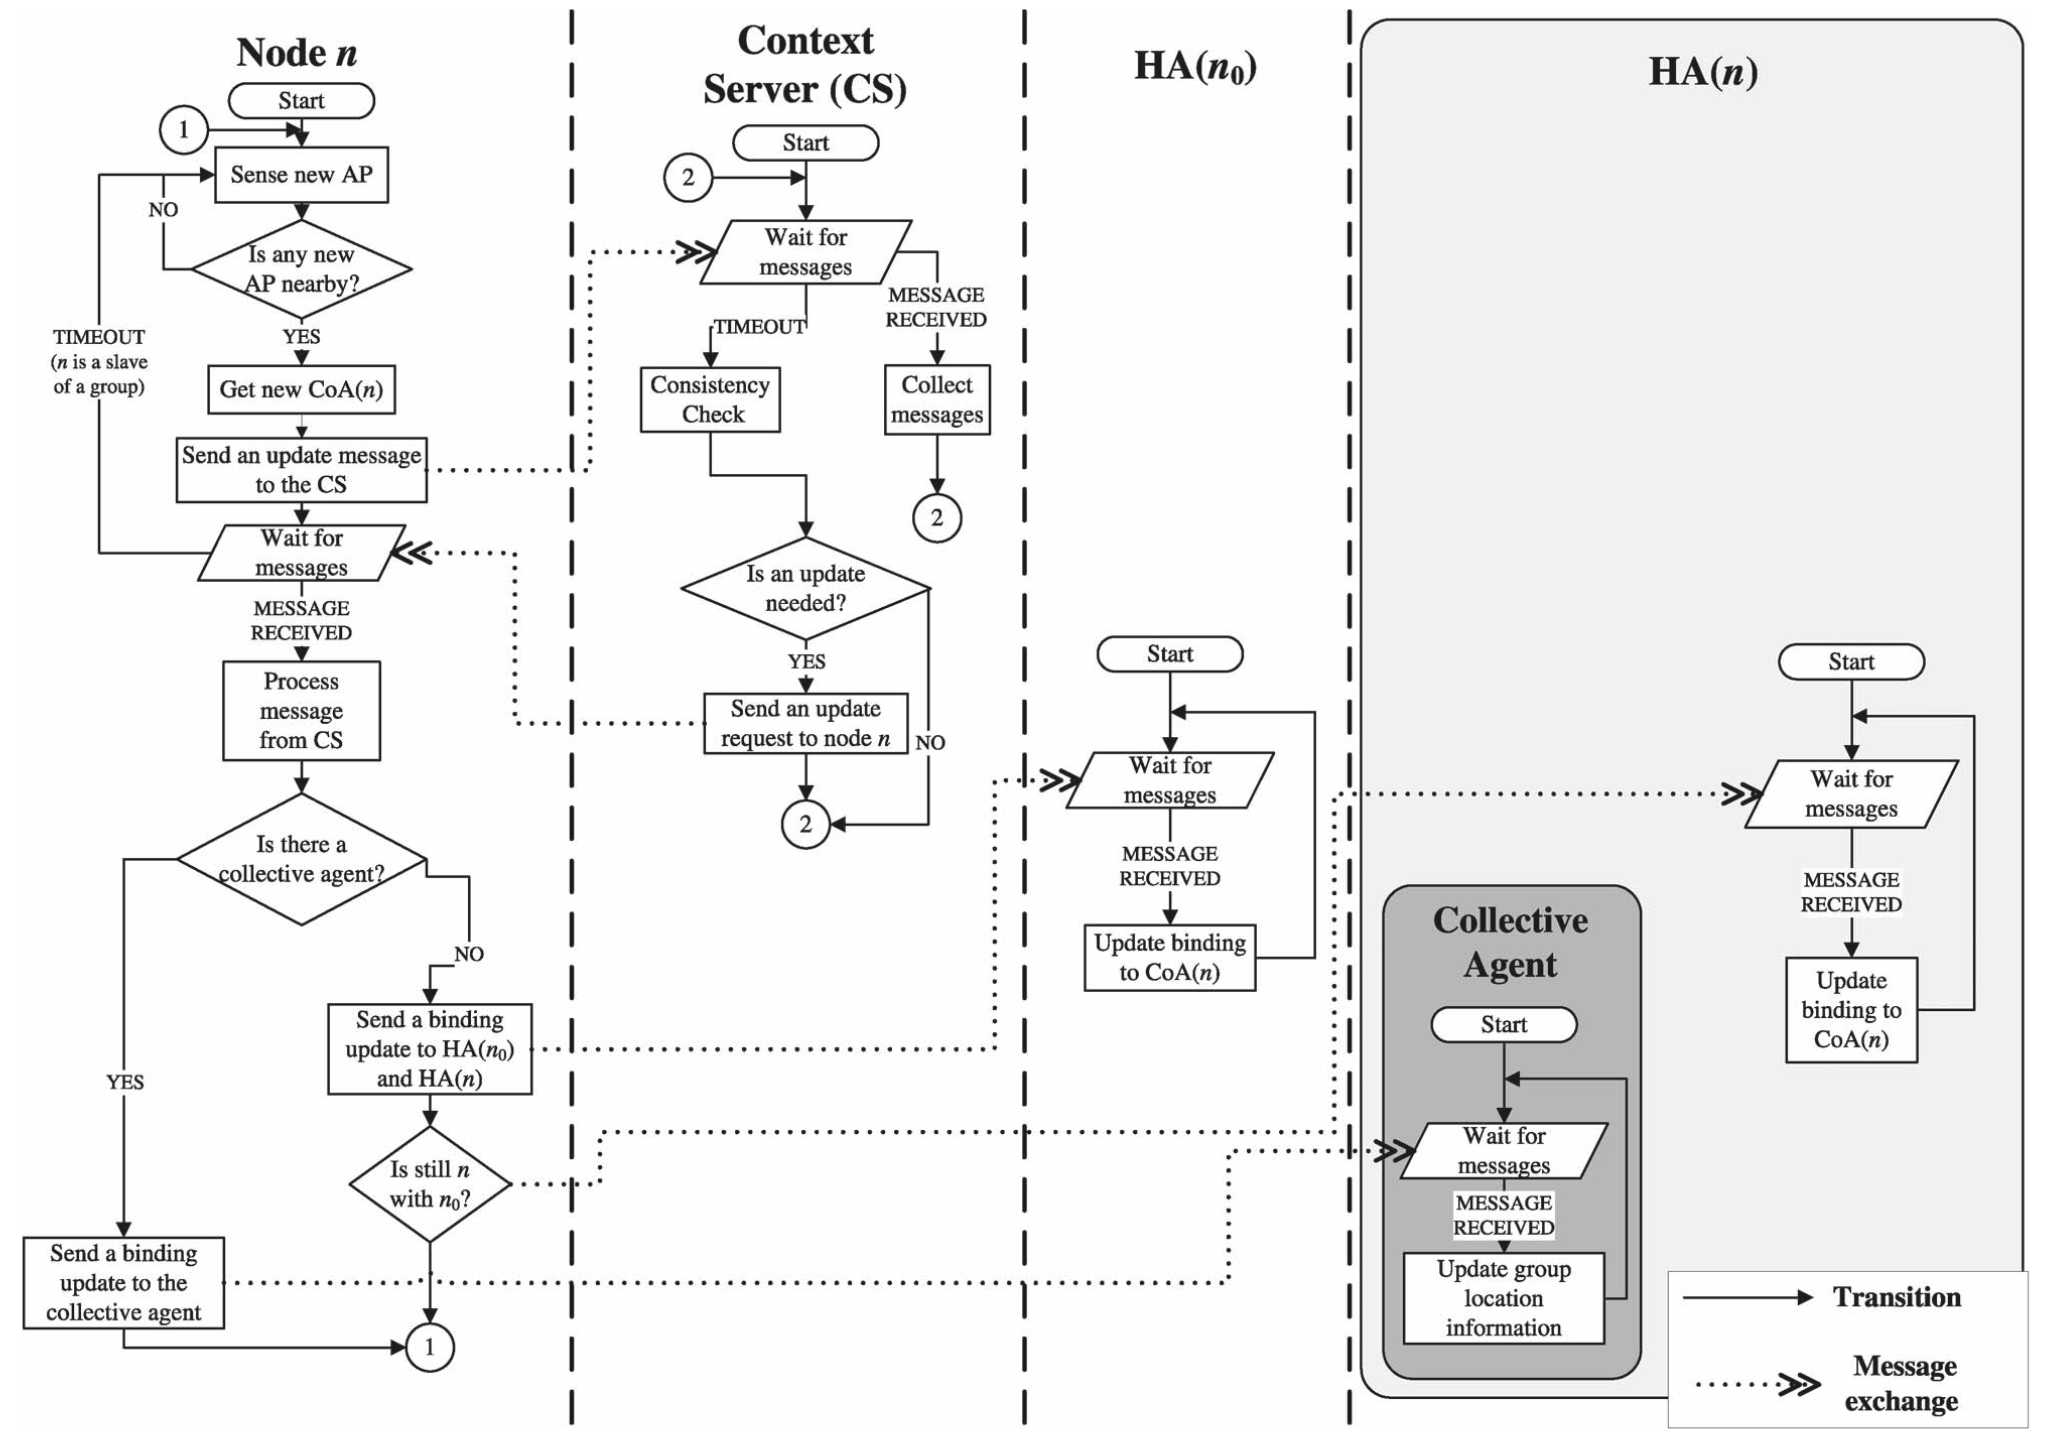
\includegraphics[width=0.9\linewidth]{figs/ogm-proc}
	\caption {فرآیند جابجایی حسگرها در OGM}
	\label{fig:ogm-proc}
\end{figure}

\section{راهکار \lr{Self Organized Things} \lr{(SoT)}}
در راهکار ارائه شده‌ی مقاله‌ی \cite{}، علاوه بر دو هدف اصلی که تا به حال درباره‌ی آن صحبت نموده‌ایم - یعنی کاهش انرژی مصرفی سیستم و به دنبال آن، افزایش طول عمر سیستم - هدف دیگری نیز مدنظر قرار گرفته است و آن کاهش نیازمندی به انسان جهت مدیریت سیستم‌های مبتنی بر اینترنت اشیا می‌باشد.
راهکار ارائه شده در این مقاله، بر اساس سه تابع \lr{Self-Configuration}، 
\lr{Self-Optimization} و \lr{Self-Healing}
رفتار می‌کند که در ادامه به بررسی هریک از آن‌ها می‌پردازیم.

\subsection{تابع \lr{Self-Configuration}}
اولین تابع به کار رفته در سازوکار ارائه شده، تابع \lr{Self-Configuration} است. این تابع همان‌گونه که در شکل \ref{fig:sot-al1} قابل مشاهده است، وظیفه‌ی پیکربندی اولیه سیستم را بر عهده دارد. عملکرد تابع مذکور به این شکل است که هر یک از حسگر‌های \lr{Trigger-Based} را در حالت فعال و تمامی حسگرهای \lr{Periodic} را در حالت خواب قرار می‌دهد. لازم به ذکر است که در این سیستم، حالت هر حسگر (که با $\phi$ نمایش داده می‌شود) بر سه نوع است. خواب\LTRfootnote{Sleep}، بیدار\LTRfootnote{Active} و منفعل (خاموش)\LTRfootnote{Passive}. در حالت خواب، حسگر روشن است اما به پایش و دریافت اطلاعات محیط مشغول نیست و در نتیجه کمترین میزان مصرف انرژی را دارد. در حالت بیدار (فعال)، حسگر روشن است و به پایش محیط می‌پردازد. در حالت خاموش نیز حسگر به طور کلی خاموش است و انرژی‌ای مصرف نمی‌کند.

\begin{figure}
	\centering
	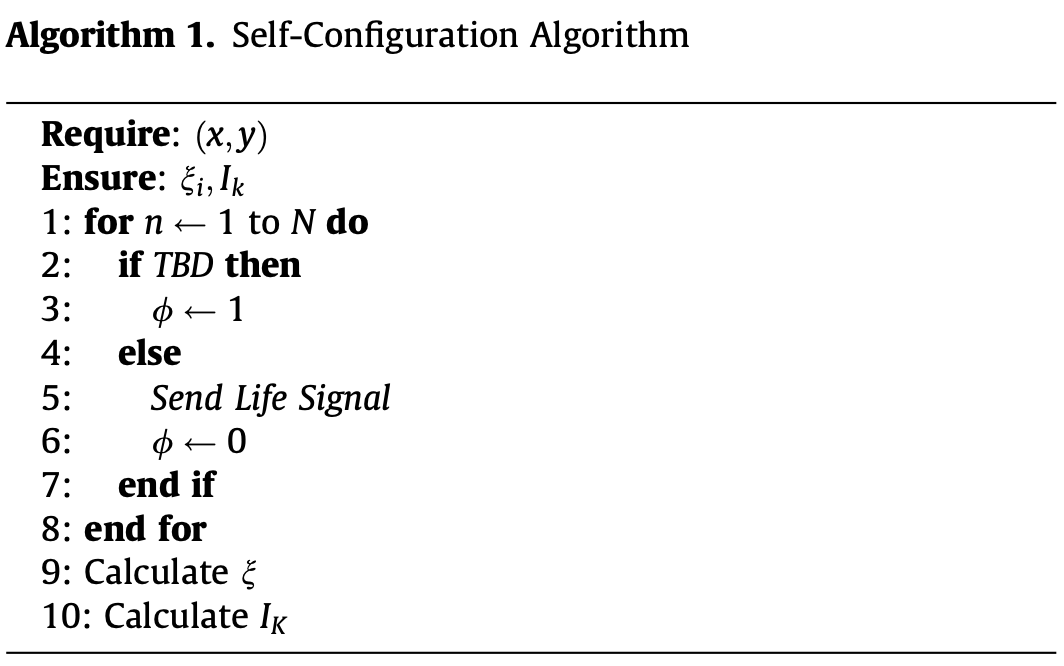
\includegraphics[width=0.7\linewidth]{figs/sot-al1}
	\caption {شبه کد تابع Self-Configuration}
	\label{fig:sot-al1}
\end{figure}

\par
پس از آن که وضعیت هر حسگر بنابر نوع آن تنظیم شد؛ همان‌طور که در خط ۹ و ۱۰ شبه کد شکل \ref{fig:sot-al1} مشاهده می‌شود؛ نوبت به محاسبه‌ی دو پارامتر تعریف شده در این مقاله به ازای هر یک از حسگر‌ها می‌رسد. در ادامه به تعریف این دو پارامتر می‌پردازیم.

\subsubsection{
محاسبه هم‌پوشانی ($\zeta_i$)
}
یکی از پارامترهای معرفی شده در مقاله‌ی مورد بررسی، پارامتری تحت عنوان هم‌پوشانی است که مشخص‌کننده‌ی این است که یک حسگر چه مساحتی را منحصرا تحت پوشش قرار داده است. نحوه‌ی محاسبه‌ی این پارامتر در فرمول \ref{eq:sot-conflict} مشاهده می‌شود. ($D_{ij}$ بیانگر فاصله‌ی بین دو گره $i$ و $j$ است.)

\begin{equation}
\zeta_i = \sum_j \frac{D_{ij} \times 1(D_{ij} < 2R) + 2R \times 1(D_{ij} \geq 2R)}{2R}
\label{eq:sot-conflict}
\end{equation}

\subsubsection{
محاسبه همبستگی فضایی ($I_k$)
}
پارامتر دیگری که در این مقاله به آن اشاره شده، پارامتر همبستگی فضایی\LTRfootnote{Spatial Correlation} می‌باشد. دلیل معرفی این پارامتر این است که پارامتر قبلی (یعنی هم‌پوشانی $\zeta_i$) به تنهایی به موقعیت مکانی حسگرها وابسته است و توجهی به وضعیت حسگرها ندارد. 




















%%%%%%%%%%%%%%%%%%%%%%%%%%%
	
%%%%%%%%%%%%%%%%%%%%%%%%
% مراجع
\newpage
%\onehalfspacing
\bibliographystyle{ieeetr-fa}%{chicago-fa}%{plainnat-fa}%
\bibliography{thesis}
%%%%%%%%%%%%%%%%%%%%%%%%

\end{document}
